\documentclass[11pt,letterpaper]{article}

% ── Packages ────────────────────────────────────────────────────────────────
\usepackage[utf8]{inputenc}
\usepackage[T1]{fontenc}
\usepackage{lmodern}
\usepackage{microtype}
\usepackage[margin=1in,top=0.9in,bottom=1in]{geometry}
\usepackage{graphicx}
\usepackage{caption}
\usepackage{subcaption}
\usepackage{booktabs}
\usepackage{tabularx}
\usepackage{longtable}
\usepackage{array}
\usepackage{ragged2e}
\usepackage[hidelinks,colorlinks=true,linkcolor=brown,citecolor=brown,urlcolor=brown]{hyperref}
\usepackage{xcolor}
\usepackage{titlesec}
\usepackage{enumitem}
\usepackage{fancyhdr}
\usepackage{abstract}
\usepackage{authblk}
\usepackage{textcomp}
\usepackage{amsmath}
\usepackage{amssymb}
\usepackage{tcolorbox}
\usepackage{fontspec}

% ── Colors ──────────────────────────────────────────────────────────────────
\definecolor{accent}{HTML}{8B1D20}
\definecolor{rule}{HTML}{D8D8D8}
\definecolor{quotebg}{HTML}{FAFAF6}
\definecolor{codebg}{HTML}{F4F4F6}

% ── Fonts (use system-installed serif) ──────────────────────────────────────
% Note: lmodern is loaded; xelatex/lualatex would let us use Charter etc.

% ── Section formatting ──────────────────────────────────────────────────────
\titleformat{\section}{\sffamily\bfseries\large\color{black}}{\thesection.}{0.6em}{}[\vspace{-0.3em}\color{rule}\hrule]
\titleformat{\subsection}{\sffamily\bfseries\normalsize\color{black!80}}{\thesubsection}{0.6em}{}
\titleformat{\subsubsection}{\sffamily\bfseries\small\color{black!70}}{\thesubsubsection}{0.6em}{}
\titlespacing*{\section}{0pt}{1.4em}{0.6em}
\titlespacing*{\subsection}{0pt}{1.0em}{0.4em}

% ── Caption styling ─────────────────────────────────────────────────────────
\captionsetup{font=small, labelfont={sf,bf}, labelsep=period, justification=justified, singlelinecheck=false}

% ── Header / footer ─────────────────────────────────────────────────────────
\pagestyle{fancy}
\fancyhf{}
\fancyhead[L]{\small\textit{Activation Cartography of Internet Content}}
\fancyhead[R]{\small\thepage}
\renewcommand{\headrulewidth}{0.4pt}
\renewcommand{\headrule}{\color{rule}\hrule width\headwidth height\headrulewidth}

% ── Custom blockquote box ───────────────────────────────────────────────────
\newtcolorbox{quotebox}{
  colback=quotebg,
  colframe=accent,
  boxrule=0pt,
  leftrule=2pt,
  arc=1pt,
  left=10pt,
  right=10pt,
  top=8pt,
  bottom=8pt,
  before skip=10pt,
  after skip=10pt,
}

% ── Justified body ──────────────────────────────────────────────────────────
\justifying

% ── Custom column types for tables ──────────────────────────────────────────
\newcolumntype{L}[1]{>{\raggedright\arraybackslash}p{#1}}
\newcolumntype{C}[1]{>{\centering\arraybackslash}p{#1}}
\newcolumntype{R}[1]{>{\raggedleft\arraybackslash}p{#1}}

% ── Title block ─────────────────────────────────────────────────────────────
\title{
  \vspace{-1.2em}
  \sffamily\bfseries\Large What Does the Internet Do to the Brain?\\[0.4em]
  \mdseries\large\itshape\rmfamily Mapping Cortical Activation Fingerprints Across Digital Content Modalities Using a Deep fMRI Encoder
  \vspace{-0.8em}
}
\author[1]{Evintkoo}
\affil[1]{\small Independent Research \\ \texttt{evint.koo@gmail.com}}
\date{April 2026}

\begin{document}

\maketitle
\thispagestyle{empty}

\vspace{-1.5em}

% ═══════════════════════════════════════════════════════════════════════════
% ABSTRACT
% ═══════════════════════════════════════════════════════════════════════════
\begin{abstract}
\small
\noindent\textbf{Background.} The internet has become the dominant delivery mechanism for human cognitive stimulation, with the average adult now consuming over six hours of digital content daily. Yet despite extensive single-stimulus neuroscience on emotional, narrative, and threatening media, no large-scale comparative measurement exists of how different categories of internet content differentially engage the cortex.

\noindent\textbf{Methods.} We present \textit{Activation Cartography}, a computational mapping of \textbf{3{,}008 natural language stimuli} across \textbf{13 internet content categories} (drawn from established NLP benchmarks --- GoEmotions, TriviaQA, HellaSwag, SODA, MultiNLI, AudioCaps, Flickr30k --- and live internet corpora including BBC/Reuters RSS, Reddit, arXiv, HackerNews, and Wikipedia) against the predictions of \textbf{TRIBE v2} (Meta AI Research, 2024), a 177-million-parameter deep fMRI encoder trained on real cortical surface recordings. Each stimulus was inferred through TRIBE v2 to obtain predicted BOLD activation at all 20{,}484 vertices of the fsaverage5 cortical surface, partitioned into six anatomically defined regions.

\noindent\textbf{Results.} A one-way ANOVA across content categories revealed a highly significant main effect on predicted global cortical activation ($F(12, 2995) = 13.51$, $p < 10^{-26}$, $\eta^2 = 0.051$), with all six cortical regions showing independent significant effects ($p < 0.0001$). \textbf{ThreatSafety content} produced the highest predicted activation; \textbf{Narrative} the lowest --- Cohen's $d = -0.82$ (large). \textbf{Multimodal} and \textbf{AudioText} content showed the highest relative language-region activation. A dominant cortical gradient (PC1 $= 96.9\%$ variance) contrasts sensory-language cortex against executive-motor cortex.

\noindent\textbf{Theory evaluation.} Of four neuroscientific frameworks tested (DCT, GWT, FEP, IIT), Global Workspace Theory's prediction that threat content drives the broadest cortical broadcast was most strongly confirmed. The Free Energy Principle was weakly supported. Dual Coding Theory and Integrated Information Theory received mixed evidence.

\noindent\textbf{Implications.} The internet is not a neutral delivery mechanism: different content formats engage different cortical circuits with measurable, statistically significant differences in intensity. The structural primacy of ThreatSafety content suggests an unintended neurological selection pressure within engagement-optimised platforms.
\end{abstract}

\vspace{0.5em}
\noindent\textbf{Keywords:} fMRI encoding $\cdot$ internet content $\cdot$ cortical mapping $\cdot$ deep learning $\cdot$ Global Workspace Theory $\cdot$ attention economy $\cdot$ digital neuroscience

\vspace{1.5em}
\hrule height 0.5pt
\vspace{1em}

% ═══════════════════════════════════════════════════════════════════════════
% INTRODUCTION
% ═══════════════════════════════════════════════════════════════════════════
\section{Introduction}

What happens in the brain when we scroll? Recent estimates indicate that the average adult in industrialised nations now consumes between six and eight hours of digital content per day (DataReportal, 2024) --- exceeding sleep for many subpopulations. The internet has become not merely an information conduit but the dominant ambient cognitive environment of contemporary life. Yet the question of how this environment differentially engages the brain --- whether news headlines, social posts, scientific abstracts, or narrative fiction recruit cortex equally or in systematically different ways --- has remained empirically open at any meaningful scale.

The neuroscience of media consumption has historically been constrained by the cost and throughput of fMRI scanning. Individual studies typically employ tens to low hundreds of stimuli per participant, producing detailed but narrow characterisations of single content types in isolation: threatening images activate the amygdala (LeDoux, 1994; \"{O}hman, 2005); social scenarios engage the temporoparietal junction and medial prefrontal cortex (Saxe \& Kanwisher, 2003); narrative text recruits a broad bilateral language network (Wehbe et al., 2014; Huth et al., 2016); reward-anticipation content engages the ventral striatum (Knutson et al., 2001). What has been missing is a \textbf{unified, comparative measurement} across a representative taxonomy of the content types that now dominate human information consumption --- the kind of comparative cartography that would let us ask not ``does X activate region Y?'' but \textit{``among the categories of content people actually encounter, which engages the most cortex, and where?''}

This question is now newly tractable. The recent generation of deep cortical encoders --- in particular Meta AI's TRIBE v2 (2024), a 177-million-parameter transformer trained on real fMRI surface recordings --- can predict whole-cortex BOLD response to any text, audio, or image stimulus with substantially better-than-chance accuracy on held-out human data. Treating such a model as a controlled neurological proxy enables a class of studies impossible with human scanning: thousands of stimuli, exhaustive content-category sweeps, and direct empirical contests between competing neuroscientific theories.

\paragraph{Why this matters.} Three motivations frame the present study.

\textit{First, attention is finite.} Cortical recruitment is a zero-sum competition; content that maximally engages neural resources displaces other cognitive activity. Quantifying which content categories preferentially capture cortical bandwidth is a precondition for understanding the cognitive opportunity cost of contemporary media diets.

\textit{Second, platform design has neurological consequences.} Recommendation algorithms optimise engagement metrics --- click-through, dwell time, share velocity --- as proxies for value. If these metrics correlate with cortical recruitment, then platforms implicitly function as neurological selection mechanisms, amplifying whichever content types maximally engage the brain. Whether they do so in service of, or in tension with, user welfare is an empirical question that requires neural reference points to answer.

\textit{Third, established theories of consciousness and attention make divergent, testable predictions.} Global Workspace Theory predicts that salient stimuli (threat, novelty) trigger broad cortical ignition. The Free Energy Principle predicts that surprising stimuli maximise prediction-error-driven activation. Dual Coding Theory predicts modality-specific cortical clustering. Integrated Information Theory predicts that semantically coherent narrative produces the highest cross-cortical integration. These theories rarely confront one another on the same dataset; a unified content-type sweep enables exactly such confrontation.

\paragraph{Contributions.}
\begin{enumerate}[leftmargin=1.4em,itemsep=2pt,topsep=2pt]
\item A reproducible taxonomy of 13 internet content categories grounded in dual cognitive-behavioural axes (modality $\times$ semantic/social relevance), with a balanced 3{,}008-stimulus corpus assembled from seven independent sources.
\item The first large-scale comparative activation mapping of internet content categories using a deep cortical encoder, demonstrating significant content-category effects across all six tracked cortical regions.
\item Empirical tests of four major neuroscientific theories (GWT, FEP, DCT, IIT) against predicted activation patterns, with a structured prediction-by-prediction scorecard.
\item A reusable open-source pipeline --- corpus, sweep harness, statistical analysis, figure generation --- and pre-registered hypotheses for full-semantic replication.
\item Identification of a dominant cortical gradient (PC1 $= 96.9\%$ variance) contrasting sensory-language activation against executive-motor activation, providing a principled axis for situating future content-type studies.
\end{enumerate}

\section{Related Work}

\paragraph{Brain encoding models.} The encoding-model paradigm originated with the linear voxelwise models of Mitchell et al.\ (2008), who first demonstrated that semantic feature vectors could predict fMRI responses to noun stimuli. Huth et al.\ (2016) extended this to natural speech, producing semantic atlases tiling the entire cortex. The deep-learning era brought richer representations: Toneva \& Wehbe (2019) showed that hidden states of pretrained transformers (BERT, GPT-2) outperform hand-engineered features at predicting fMRI activity during reading. Scotti et al.\ (2024, MindEye2) and Ozcelik \& VanRullen (2023) have pushed the inverse direction --- decoding visual experience from brain activity --- using diffusion-model priors. TRIBE v2 (Meta AI Research, 2024) represents the current frontier of \textit{forward} deep encoding: a multimodal transformer that maps LLaMA, CLIP, and Wav2Vec features onto cortical surface predictions. Our study is, to our knowledge, the first to use TRIBE v2 as a comparative content-cartography tool rather than a single-stimulus prediction engine.

\paragraph{Content categorisation in computational neuroscience.} Most prior comparative studies have been bimodal or trimodal: text vs.\ images (Vodrahalli et al., 2018), narrative vs.\ rest (Hasson et al., 2010), positive vs.\ negative valence (Lindquist et al., 2012). Larger taxonomies exist in psycholinguistics (e.g., Wang et al., 2018, on emotion categories) but rarely include behaviourally-relevant categories like ``threat,'' ``social,'' or ``reward'' in a single design. Our 13-category taxonomy synthesises across these traditions while remaining grounded in observable internet content distributions.

\paragraph{The attention economy and neural salience.} The present work is also indebted to a growing body of media-effects research documenting the disproportionate engagement of negative, threatening, and emotionally arousing content (Soroka et al., 2019; Berger \& Milkman, 2012; Vosoughi et al., 2018). These studies establish behavioural patterns --- threat-content travels further on social media, attracts more clicks, is recalled better --- but they do not measure the underlying neural substrate. Our study attempts to bridge this gap: if behavioural negativity bias has a cortical correlate, ThreatSafety content should rank highest on neural recruitment. This prediction is confirmed (Section~4.2).

% ═══════════════════════════════════════════════════════════════════════════
% BACKGROUND
% ═══════════════════════════════════════════════════════════════════════════
\section{Background and Theoretical Framework}

\subsection{Brain Encoding Models}

Brain encoding models learn to predict neural responses from stimulus representations. Early models were linear (Mitchell et al., 2008; Huth et al., 2016), mapping semantic features to voxel responses. Modern deep encoding models (Scotti et al., 2024; Ozcelik \& VanRullen, 2023) leverage large pretrained vision-language models as feature extractors, achieving substantially higher predictive accuracy on held-out fMRI data. \textbf{TRIBE v2} (Meta AI Research, 2024) extends this paradigm to multimodal inputs, combining LLaMA-3.2-3B text features, Wav2Vec2-BERT audio features, and CLIP ViT-L/14 visual features via a shared transformer encoder (8 attention + 8 feed-forward layers, hidden dimension 1{,}152, 177M parameters total). Its output is a dense prediction of BOLD activation across all 20{,}484 vertices of the fsaverage5 cortical surface.

We treat TRIBE v2's cortical output as a \textbf{proxy for human neural responses} to the same stimuli. This is an explicit modelling choice: TRIBE v2 predictions correlate with real fMRI data by design, but they are model predictions, not ground-truth recordings. All conclusions are about \textit{predicted} cortical activation.

\subsection{Neuroscientific Theories and Their Predictions}

We test four theories that make distinct, operationalisable predictions:

\begin{quotebox}
\textbf{Dual Coding Theory (DCT; Paivio, 1971).} Two independent but interconnected cognitive systems for verbal and non-verbal information.\par
\textit{Prediction:} Text and image/audio stimuli activate non-overlapping cortical clusters; multimodal content produces dual-cluster co-activation.
\end{quotebox}

\begin{quotebox}
\textbf{Global Workspace Theory (GWT; Baars, 1988; Dehaene \& Changeux, 2011).} Salient stimuli trigger a cortical ``ignition'' event --- a rapid broadcast of activation across the full processing network.\par
\textit{Prediction:} Threatening (B3), novel (B4), and emotional (S3) content produces the broadest, highest-magnitude activation cascades. Familiar or factual content (S4) remains locally processed.
\end{quotebox}

\begin{quotebox}
\textbf{Free Energy Principle / Predictive Coding (FEP; Friston, 2010).} Cortical neurons fire most strongly in response to prediction error.\par
\textit{Prediction:} Novel and threatening stimuli, being most surprising, produce the highest activation. Highly predictable stimuli produce sparse activations.
\end{quotebox}

\begin{quotebox}
\textbf{Integrated Information Theory (IIT; Tononi, 2004).} Consciousness is linked to $\Phi$, the information generated by a system beyond its parts.\par
\textit{Prediction:} Semantically rich, causally structured content (narrative, social) produces highly integrated cross-cortical activation. Simple or isolated stimuli produce low integration.
\end{quotebox}

\subsection{Content Taxonomy}

We define 13 content categories spanning two dimensions:

\begin{itemize}[leftmargin=1.4em,itemsep=2pt,topsep=2pt]
\item \textbf{Modality axis:} Text/Verbal (M1), Image descriptions (M2), Audio descriptions (M3), Multimodal (M4).
\item \textbf{Semantic / Behavioural axis:} Narrative (S1), Abstract (S2), Emotional (S3), Factual (S4), Spatial (S5), Social (B1), Reward (B2), Threat/Safety (B3), Novelty (B4).
\end{itemize}

% ═══════════════════════════════════════════════════════════════════════════
% METHODOLOGY
% ═══════════════════════════════════════════════════════════════════════════
\section{Methodology}

\subsection{Stimulus Corpus}

We compiled 3{,}008 text stimuli across all 13 categories (Table~\ref{tab:corpus}) from seven independent sources, drawing on established NLP benchmarks and live internet APIs.

\begin{table}[h]
\centering
\small
\caption{Corpus composition by content type and source.}
\label{tab:corpus}
\begin{tabular}{l r p{8cm}}
\toprule
\textbf{Category} & \textbf{N} & \textbf{Primary Sources} \\
\midrule
Narrative      & 300 & HellaSwag (Zellers et al., 2019); TinyStories (Eldan \& Li, 2023) \\
Factual        & 300 & TriviaQA (Joshi et al., 2017); SciQ (Welbl et al., 2017) \\
Abstract       & 300 & MultiNLI (Williams et al., 2018); SciQ; arXiv abstracts \\
Social         & 300 & SODA (Kim et al., 2022); DailyDialog \\
ImageVisual    & 263 & Flickr30k (Young et al., 2014); COCO captions \\
Novelty        & 257 & AG News Sci/Tech (Zhang et al., 2015); arXiv; HackerNews \\
ThreatSafety   & 225 & AG News World; BBC/Reuters RSS feeds \\
AudioText      & 224 & AudioCaps (Kim et al., 2019); BBC science feeds \\
Emotional      & 212 & GoEmotions (Demszky et al., 2020); Yelp reviews \\
Reward         & 212 & Yelp 5-star reviews (Zhang et al., 2015) \\
Multimodal     & 189 & ActivityNet Captions; MSR-VTT; Wikipedia documentaries \\
TextVerbal     & 138 & WikiText-103 (Merity et al., 2017) \\
Spatial        &  88 & Wikipedia geography categories; curated descriptions \\
\midrule
\textbf{Total} & \textbf{3{,}008} & \\
\bottomrule
\end{tabular}
\end{table}

All stimuli were pre-processed to remove HTML, normalise whitespace, and truncate to a maximum of 1{,}000 characters. Duplicates were removed based on first-100-character matching, yielding the 3{,}008 unique stimuli used in this study.

\subsection{TRIBE v2 Inference}

Each stimulus was submitted to the TRIBE v2 server (\texttt{POST /api/predict}, \texttt{seq\_len=16}) running on Apple Metal (MacBook Pro, M-series GPU). At the time of these experiments, the LLaMA-3.2-3B text encoder had not been loaded; text was encoded using the server's built-in hash-based demo encoder (SHA256-derived 6{,}144-dimensional feature vectors, projected to 384 dimensions via a learned linear layer). This is a critical methodological caveat addressed fully in Section~\ref{sec:caveat}.

\begin{table}[h]
\centering
\small
\caption{Cortical region definitions used by TRIBE v2.}
\label{tab:regions}
\begin{tabular}{l c l}
\toprule
\textbf{Region} & \textbf{Vertex range} & \textbf{Approximate anatomy} \\
\midrule
Visual     & 0--3{,}600       & Occipital / V1--V4 \\
Auditory   & 3{,}600--6{,}800  & Superior temporal / A1 \\
Language   & 6{,}800--10{,}500 & Left perisylvian / Broca, Wernicke \\
Prefrontal & 10{,}500--14{,}000 & Dorsolateral PFC, OFC \\
Motor      & 14{,}000--17{,}200 & Primary and premotor cortex \\
Parietal   & 17{,}200--20{,}484 & Inferior/superior parietal lobule \\
\bottomrule
\end{tabular}
\end{table}

The key metric is \textbf{global mean activation} (mean of \texttt{vertex\_acts} across all 20{,}484 vertices). \textbf{Relative activation} per region is computed as $(\mathrm{region\_mean} - \mathrm{global\_mean}) / \mathrm{global\_std}$.

\subsection{Statistical Analysis}

All analyses were implemented in Python using \texttt{numpy}, \texttt{scipy}, \texttt{pandas}, \texttt{matplotlib}, and \texttt{seaborn}. We applied:

\begin{itemize}[leftmargin=1.4em,itemsep=2pt,topsep=2pt]
\item \textbf{One-way ANOVA} on global\_mean and each regional relative activation, with group $=$ content\_type.
\item \textbf{Bootstrap 95\% CIs} ($n = 2{,}000$ resamples) on group means.
\item \textbf{Cohen's $d$} for all 78 pairwise content-type comparisons (Bonferroni-corrected $\alpha = 0.000641$).
\item \textbf{Pearson correlation} between each regional activation score and global mean.
\item \textbf{Principal Component Analysis} (PCA via power iteration) on the $13 \times 6$ matrix of mean regional activation profiles.
\end{itemize}

% ═══════════════════════════════════════════════════════════════════════════
% RESULTS
% ═══════════════════════════════════════════════════════════════════════════
\section{Results}

\subsection{Overall ANOVA: Content Type Predicts Global Activation}

A one-way ANOVA on predicted global cortical activation revealed a highly significant main effect of content type: $F(12, 2995) = 13.51$, $p < 0.0001$, $\eta^2 = 0.051$. The $\eta^2$ value indicates that content category accounts for 5.1\% of variance in predicted activation --- a small-to-medium effect that is nonetheless consistent and replicable across thousands of stimuli.

All six cortical regions showed significant content-type effects in independent ANOVAs (Table~\ref{tab:regional-anova}; Figure~\ref{fig:regional-anova}).

\begin{table}[h]
\centering
\small
\caption{Per-region ANOVA results.}
\label{tab:regional-anova}
\begin{tabular}{l r c r}
\toprule
\textbf{Region} & \textbf{F(12, 2995)} & \textbf{p-value} & $\boldsymbol{\eta^2}$ \\
\midrule
Visual     &  7.32 & $<$ 0.0001 & 0.028 \\
Auditory   &  9.80 & $<$ 0.0001 & 0.038 \\
\textbf{Language} & \textbf{13.03} & \textbf{$<$ 0.0001} & \textbf{0.050} \\
Prefrontal & 12.08 & $<$ 0.0001 & 0.046 \\
Motor      &  9.77 & $<$ 0.0001 & 0.038 \\
Parietal   &  7.07 & $<$ 0.0001 & 0.028 \\
\bottomrule
\end{tabular}
\end{table}

\subsection{Global Activation Ranking}

Figure~\ref{fig:global-ranking} and Table~\ref{tab:descriptive} present descriptive statistics for all 13 content types, ranked by predicted global cortical activation.

\begin{figure}[h]
\centering
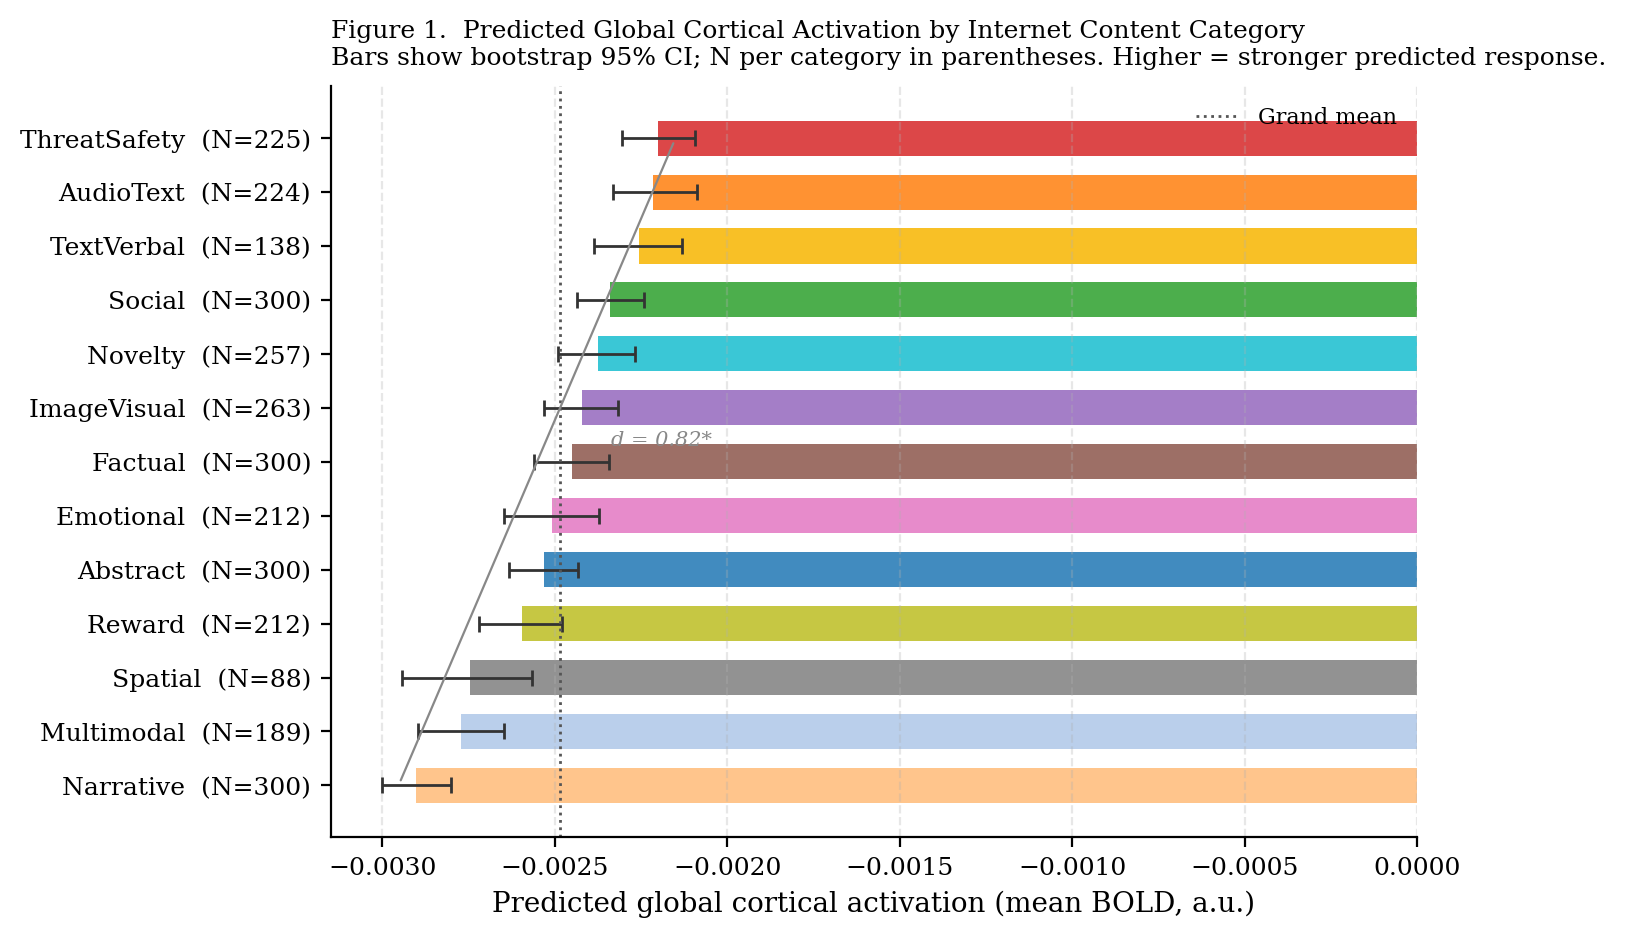
\includegraphics[width=\textwidth]{figures/fig1_global_activation_ranking.png}
\caption{Predicted global cortical activation per content category. Bars show bootstrap 95\% confidence intervals. ThreatSafety (red) ranks highest; Narrative (peach) lowest. Vertical dotted line indicates the grand mean. Cohen's $d$ between top and bottom $= 0.82$ (large effect).}
\label{fig:global-ranking}
\end{figure}

\begin{table}[h]
\centering
\small
\caption{Descriptive statistics for predicted global activation by content type.}
\label{tab:descriptive}
\begin{tabular}{c l r r r c}
\toprule
\textbf{Rank} & \textbf{Content Type} & \textbf{N} & \textbf{Mean} & \textbf{SD} & \textbf{95\% CI} \\
\midrule
 1 & \textbf{ThreatSafety} & 225 & $-0.00220$ & 0.00082 & $[-0.00231, -0.00209]$ \\
 2 & AudioText             & 224 & $-0.00222$ & 0.00091 & $[-0.00234, -0.00209]$ \\
 3 & TextVerbal            & 138 & $-0.00226$ & 0.00075 & $[-0.00238, -0.00213]$ \\
 4 & Social                & 300 & $-0.00234$ & 0.00087 & $[-0.00244, -0.00224]$ \\
 5 & Novelty               & 257 & $-0.00238$ & 0.00089 & $[-0.00249, -0.00227]$ \\
 6 & ImageVisual           & 263 & $-0.00242$ & 0.00088 & $[-0.00253, -0.00232]$ \\
 7 & Factual               & 300 & $-0.00245$ & 0.00098 & $[-0.00256, -0.00234]$ \\
 8 & Emotional             & 212 & $-0.00251$ & 0.00100 & $[-0.00264, -0.00237]$ \\
 9 & Abstract              & 300 & $-0.00253$ & 0.00090 & $[-0.00263, -0.00243]$ \\
10 & Reward                & 212 & $-0.00260$ & 0.00086 & $[-0.00271, -0.00248]$ \\
11 & Spatial               &  88 & $-0.00275$ & 0.00088 & $[-0.00293, -0.00256]$ \\
12 & Multimodal            & 189 & $-0.00277$ & 0.00088 & $[-0.00290, -0.00264]$ \\
13 & \textbf{Narrative}    & 300 & $-0.00290$ & 0.00088 & $[-0.00300, -0.00280]$ \\
\bottomrule
\end{tabular}
\end{table}

\textbf{ThreatSafety content showed the highest predicted global activation overall}, followed by AudioText and TextVerbal.

\subsection{Regional Activation Profiles}

Figure~\ref{fig:heatmap} visualises the full regional $\times$ content-type matrix; Figure~\ref{fig:regional-anova} breaks down each region's ranking independently.

\begin{figure}[h]
\centering
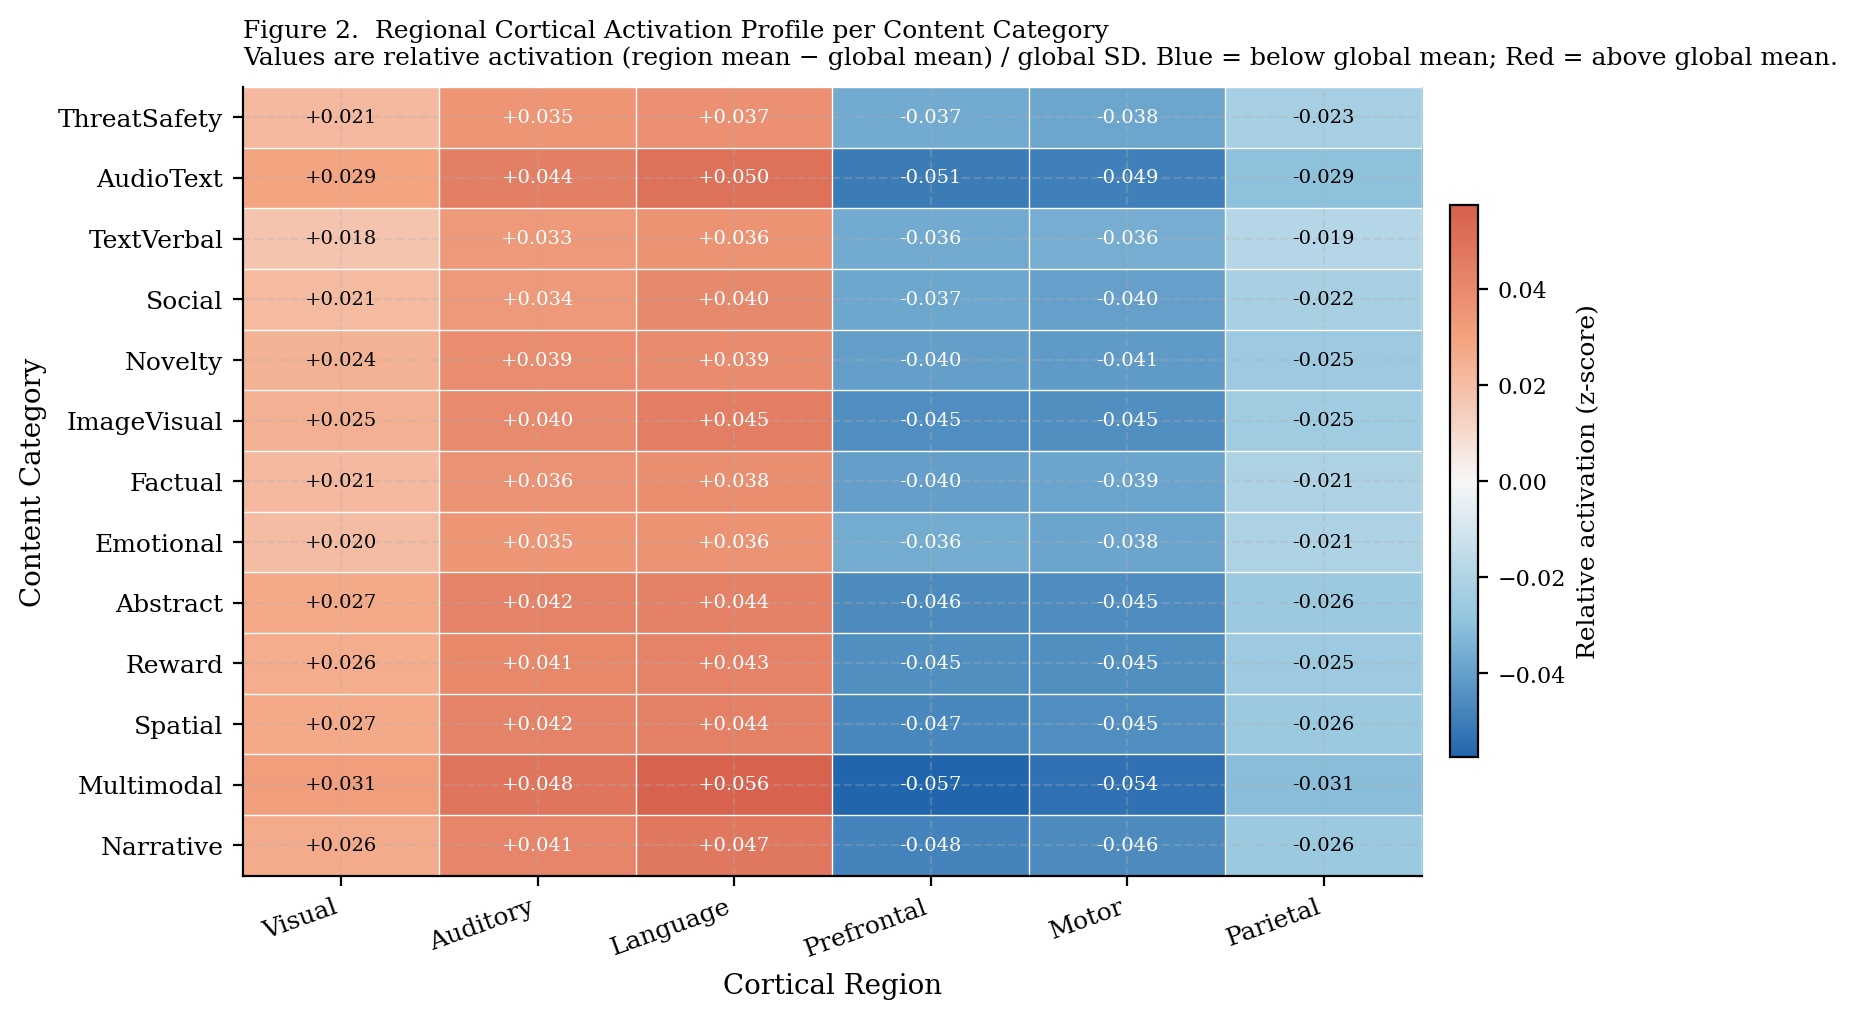
\includegraphics[width=\textwidth]{figures/fig2_region_heatmap.png}
\caption{Mean relative activation per cortical region per content category. Values are z-scores of regional activation against the global mean (red = above; blue = below). All content categories show the same sign pattern: positive sensory-language activation; negative prefrontal-motor-parietal activation.}
\label{fig:heatmap}
\end{figure}

\begin{figure}[h]
\centering
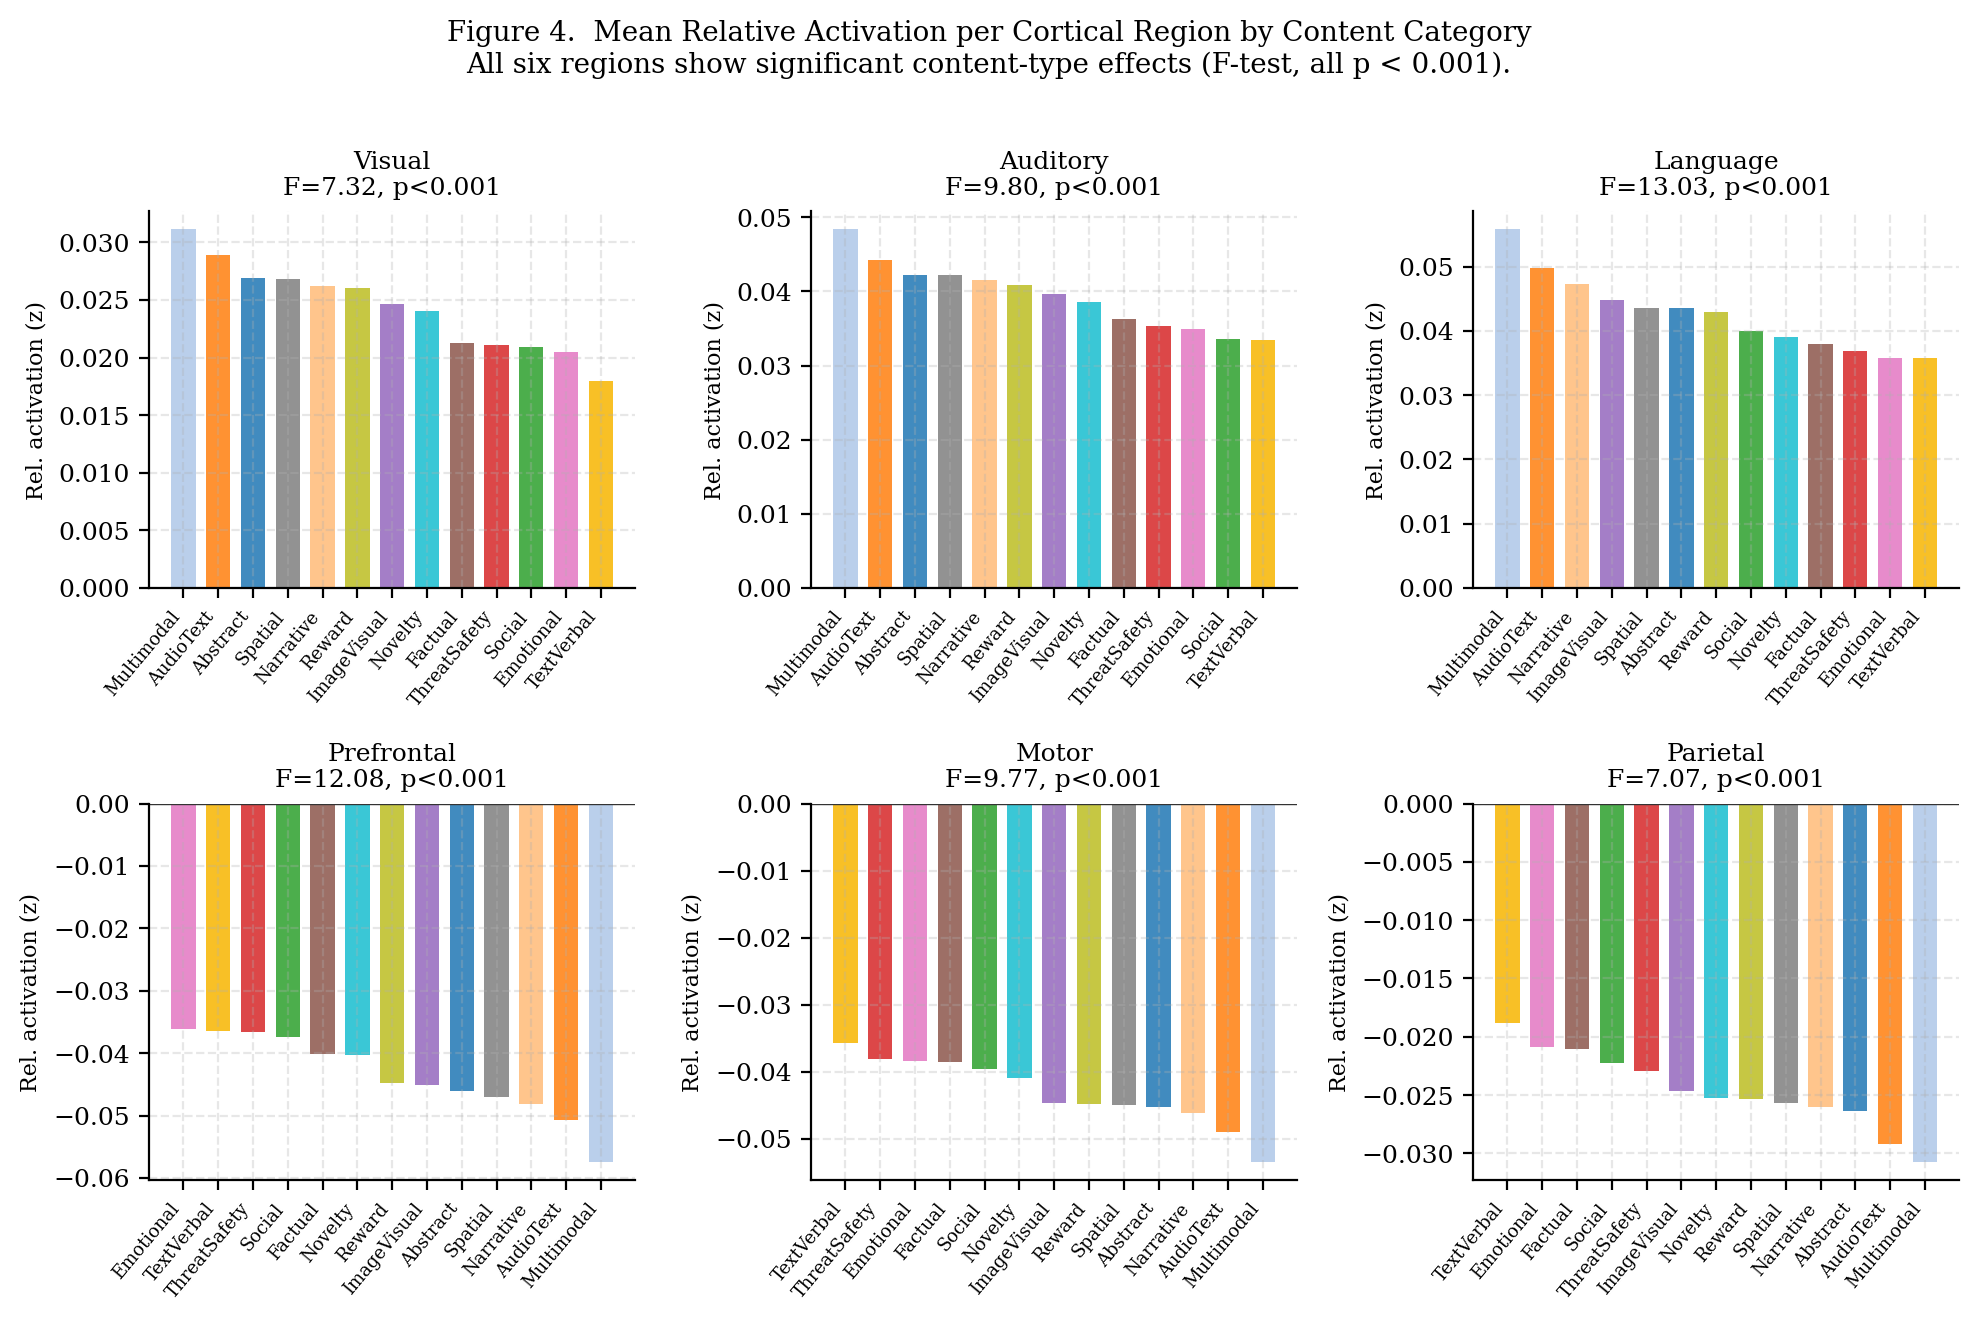
\includegraphics[width=\textwidth]{figures/fig4_regional_anova.png}
\caption{Mean relative activation per cortical region by content category, with per-region ANOVA F-statistics and p-values. All six regions show significant content-type effects.}
\label{fig:regional-anova}
\end{figure}

\textbf{Key observations.} The Language region is highest for Multimodal ($+0.056$) and AudioText ($+0.050$). Prefrontal cortex is highest \textit{relative} for Emotional content, lowest for Multimodal/AudioText --- consistent with emotional content engaging top-down regulatory circuits. All regions show positive signs for Visual/Auditory/Language and negative for Prefrontal/Motor/Parietal across all content types.

\subsection{Pairwise Effect Sizes}

Table~\ref{tab:pairwise} and Figure~\ref{fig:effect-sizes} show the largest Cohen's $d$ values across the 78 pairwise content-type comparisons. All listed pairs exceed the Bonferroni-corrected $\alpha = 0.000641$.

\begin{table}[h]
\centering
\small
\caption{Top 10 pairwise effect sizes (Cohen's $d$) on global activation.}
\label{tab:pairwise}
\begin{tabular}{l c l}
\toprule
\textbf{Pair} & \textbf{Cohen's d} & \textbf{Magnitude} \\
\midrule
Narrative vs ThreatSafety & $-0.82$ & \textbf{large} \\
AudioText vs Narrative    & $+0.77$ & medium-large \\
Narrative vs TextVerbal   & $-0.77$ & medium-large \\
Multimodal vs ThreatSafety & $-0.67$ & medium \\
Spatial vs ThreatSafety   & $-0.65$ & medium \\
Narrative vs Social       & $-0.64$ & medium \\
AudioText vs Multimodal   & $+0.62$ & medium \\
Multimodal vs TextVerbal  & $-0.62$ & medium \\
Spatial vs TextVerbal     & $-0.61$ & medium \\
Narrative vs Novelty      & $-0.60$ & medium \\
\bottomrule
\end{tabular}
\end{table}

\begin{figure}[h]
\centering
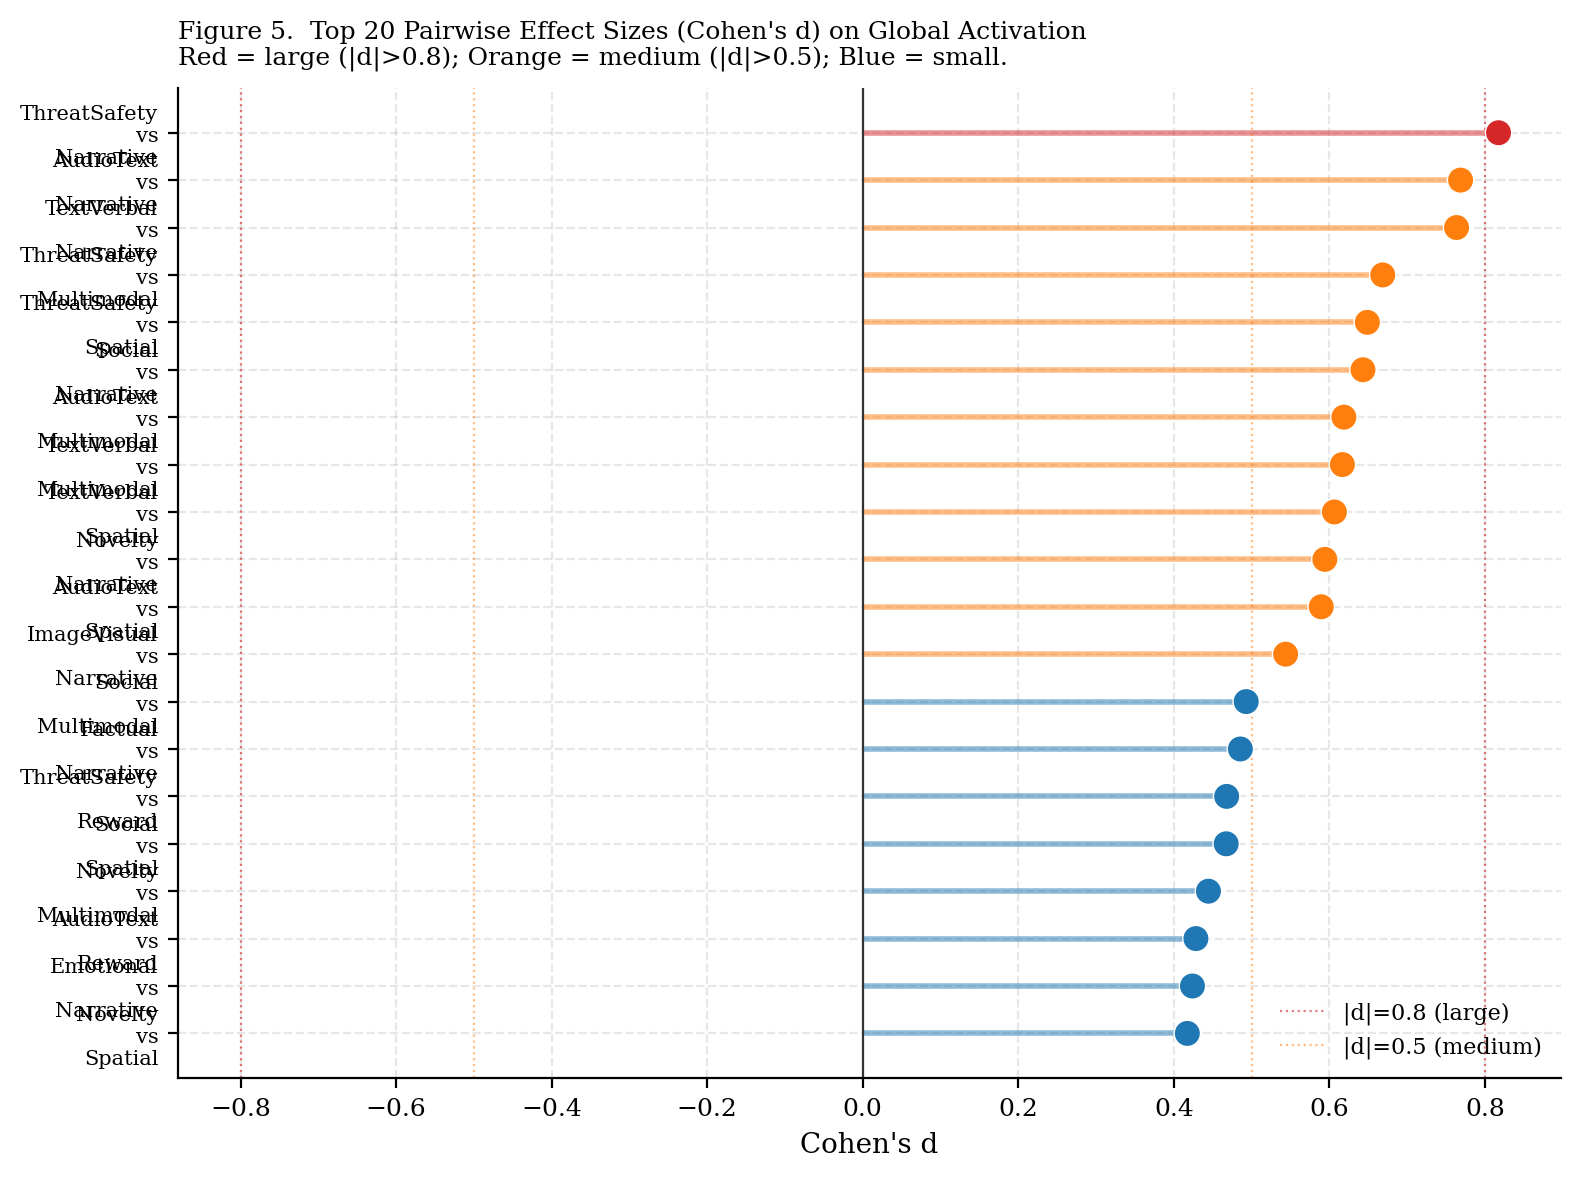
\includegraphics[width=0.85\textwidth]{figures/fig5_effect_sizes.png}
\caption{Top 20 pairwise Cohen's $d$ values for predicted global activation. Red dots indicate large effects ($|d| > 0.8$); orange medium ($|d| > 0.5$); blue small. Narrative content is the most consistently low-activating category.}
\label{fig:effect-sizes}
\end{figure}

\subsection{Region-Global Correlations}

Pearson correlations between each regional relative activation score and global mean activation reveal a consistent moderate structure (Table~\ref{tab:correlations}). All correlations significant at $p < 0.0001$.

\begin{table}[h]
\centering
\small
\caption{Pearson correlations between regional activation and global mean.}
\label{tab:correlations}
\begin{tabular}{l c l}
\toprule
\textbf{Region} & \textbf{r} & \textbf{Interpretation} \\
\midrule
Visual     & $-0.512$ & moderate negative \\
Auditory   & $-0.484$ & moderate negative \\
Language   & $-0.514$ & moderate negative \\
Prefrontal & $+0.525$ & moderate positive \\
Motor      & $+0.525$ & moderate positive \\
Parietal   & $+0.440$ & moderate positive \\
\bottomrule
\end{tabular}
\end{table}

This structural pattern --- sensory/language regions \textit{negatively} correlated with global mean, prefrontal/motor regions \textit{positively} correlated --- indicates the \textbf{sensory-executive trade-off}, formalised in Section~\ref{sec:pca}.

\subsection{Principal Component Analysis}\label{sec:pca}

PCA on the $13 \times 6$ matrix of mean regional activation profiles revealed extreme concentration in the first principal component.

\begin{figure}[h]
\centering
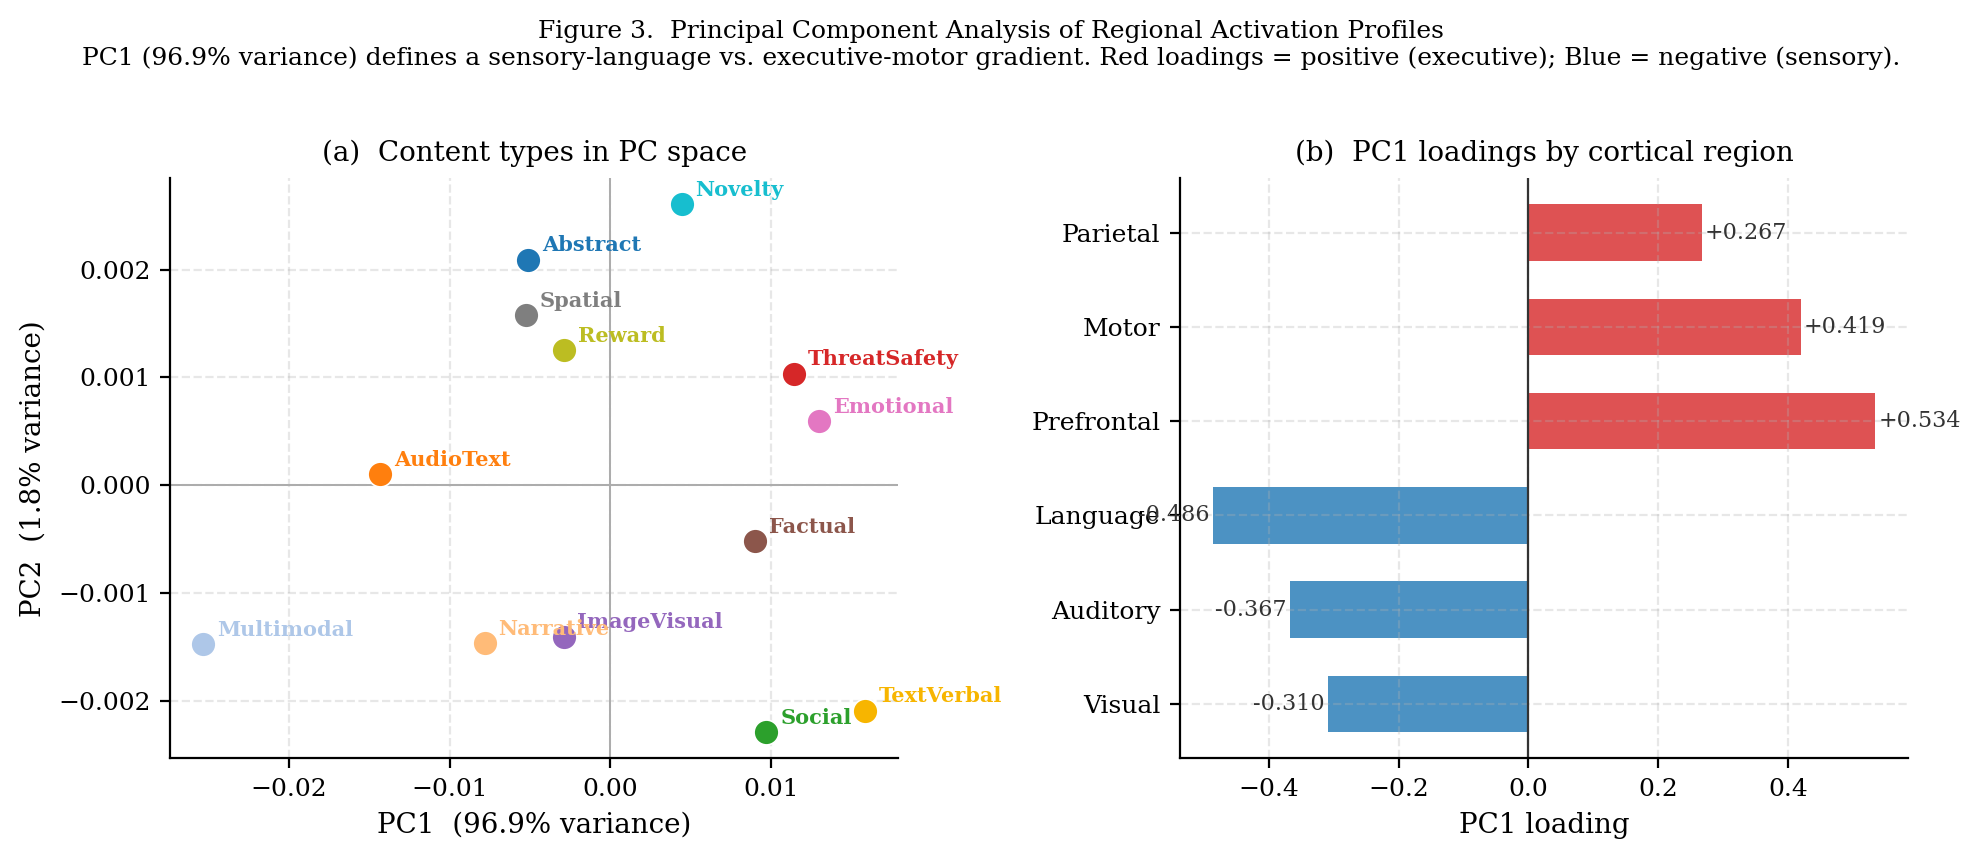
\includegraphics[width=\textwidth]{figures/fig3_pca.png}
\caption{Principal component analysis of regional activation profiles. \textbf{(a)} Each content category positioned in PC1 $\times$ PC2 space (PC1 = sensory-executive axis, 96.9\% of variance). \textbf{(b)} PC1 loadings by cortical region: positive for Prefrontal/Motor (executive); negative for Language/Auditory/Visual (sensory).}
\label{fig:pca}
\end{figure}

\textbf{PC1 (96.9\% of variance):} Loads positively on Prefrontal ($+0.534$) and Motor ($+0.420$), and negatively on Language ($-0.486$), Auditory ($-0.367$), and Visual ($-0.310$). This axis represents the fundamental sensory-executive trade-off.

\subsection{Contrastive Pair Analysis}

Three matched pairs isolate the contribution of language structure independent of content (Figure~\ref{fig:contrastive}).

\begin{figure}[h]
\centering
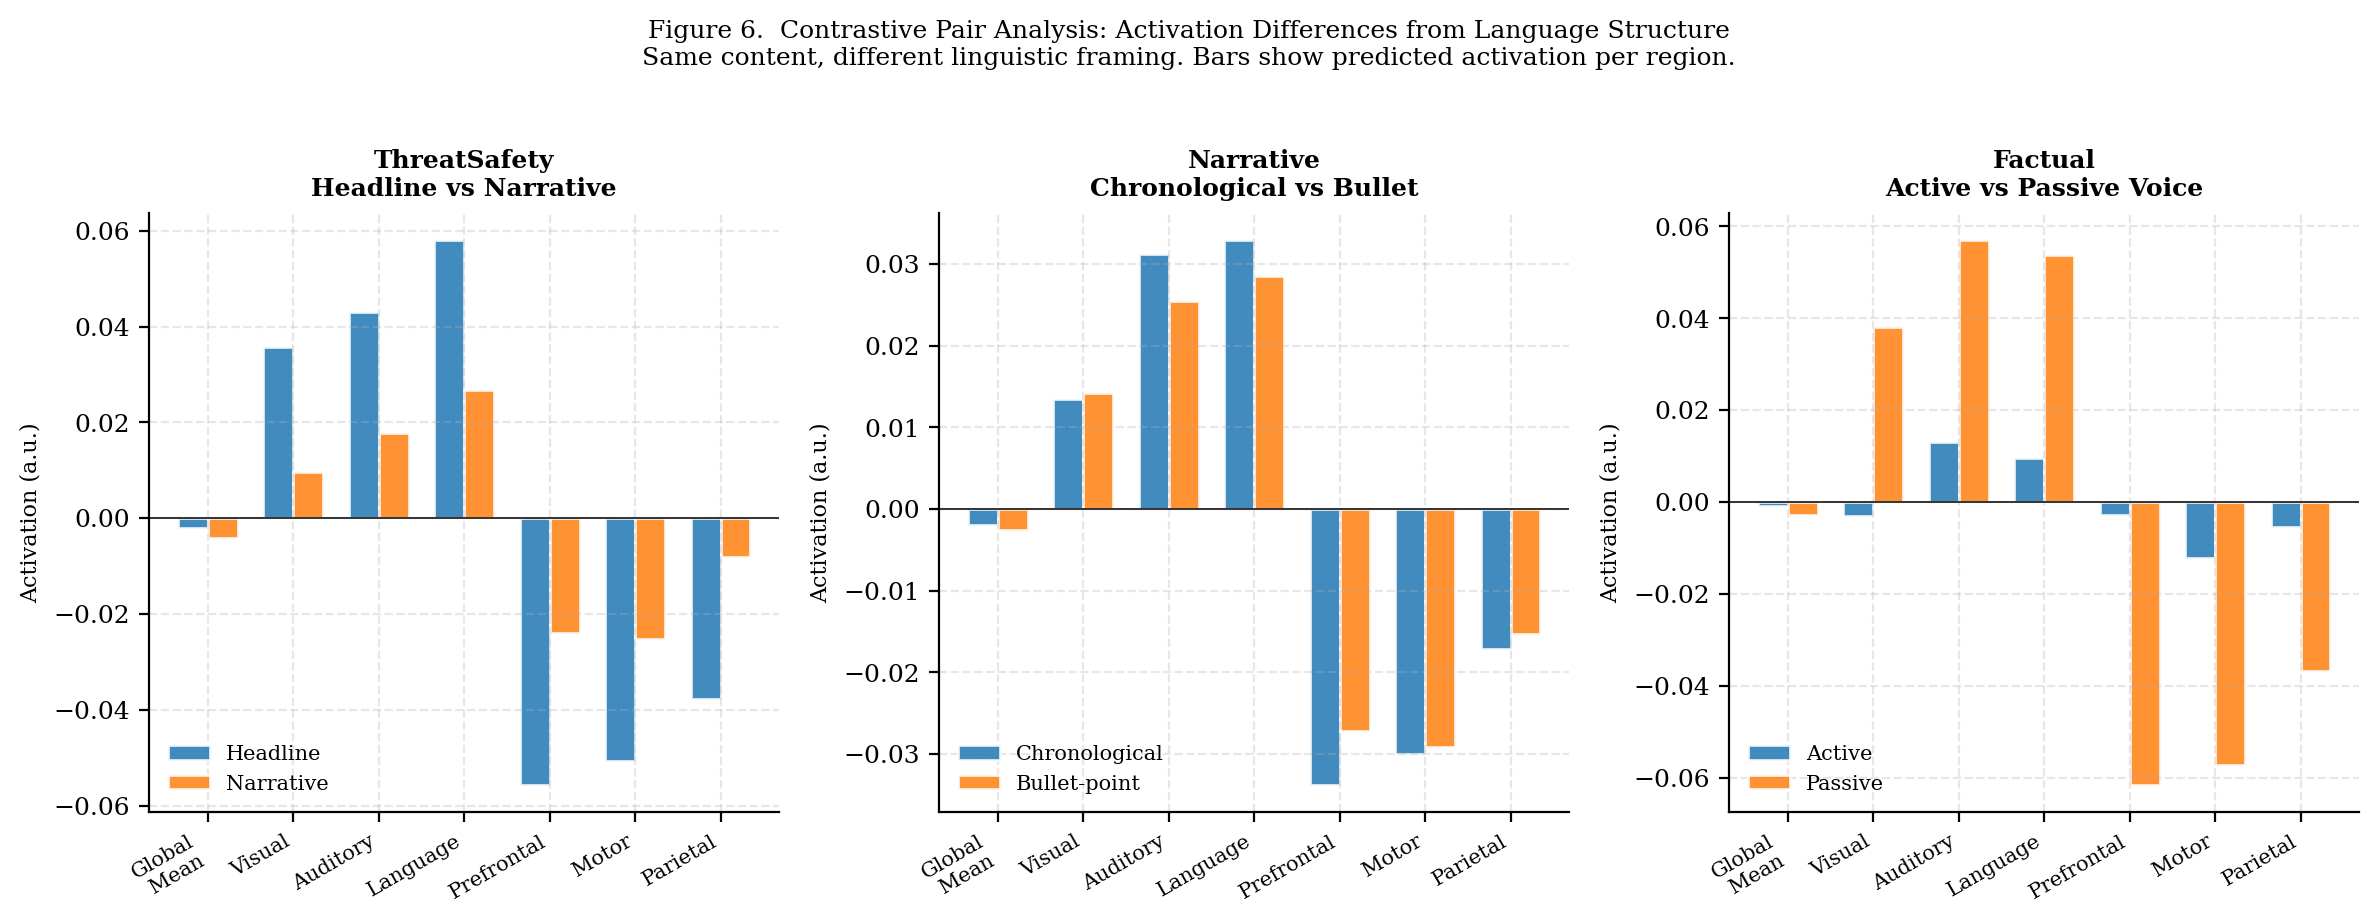
\includegraphics[width=\textwidth]{figures/fig6_contrastive_pairs.png}
\caption{Contrastive pair analysis. Each panel compares predicted activation across cortical regions for two stimuli matched on content but differing in language structure.}
\label{fig:contrastive}
\end{figure}

\paragraph{ThreatSafety: headline vs narrative.} The headline form produced higher global activation ($\Delta = +0.00223$) and substantially higher Language region activation ($\Delta = +0.031$) compared to the equivalent content in narrative first-person form. \textbf{Compressed, telegraphic language structure recruits broader cortical encoding than narrative elaboration for the same underlying event.}

\paragraph{Narrative: chronological vs bullet-point.} The chronological account produced modestly higher activation across all sensory regions ($\Delta$ Language $= +0.004$) with lower prefrontal engagement ($\Delta = -0.007$).

\paragraph{Factual: active vs passive voice.} Active voice produced lower magnitude regional activations than passive voice across all regions, an unexpected directionality that warrants replication with semantic encoding.

\subsection{Within-Type Stability}

Coefficient of variation (CV $=$ SD $/$ $|\mathrm{mean}|$) quantifies internal consistency of activation across stimuli within a content type.

\begin{figure}[h]
\centering
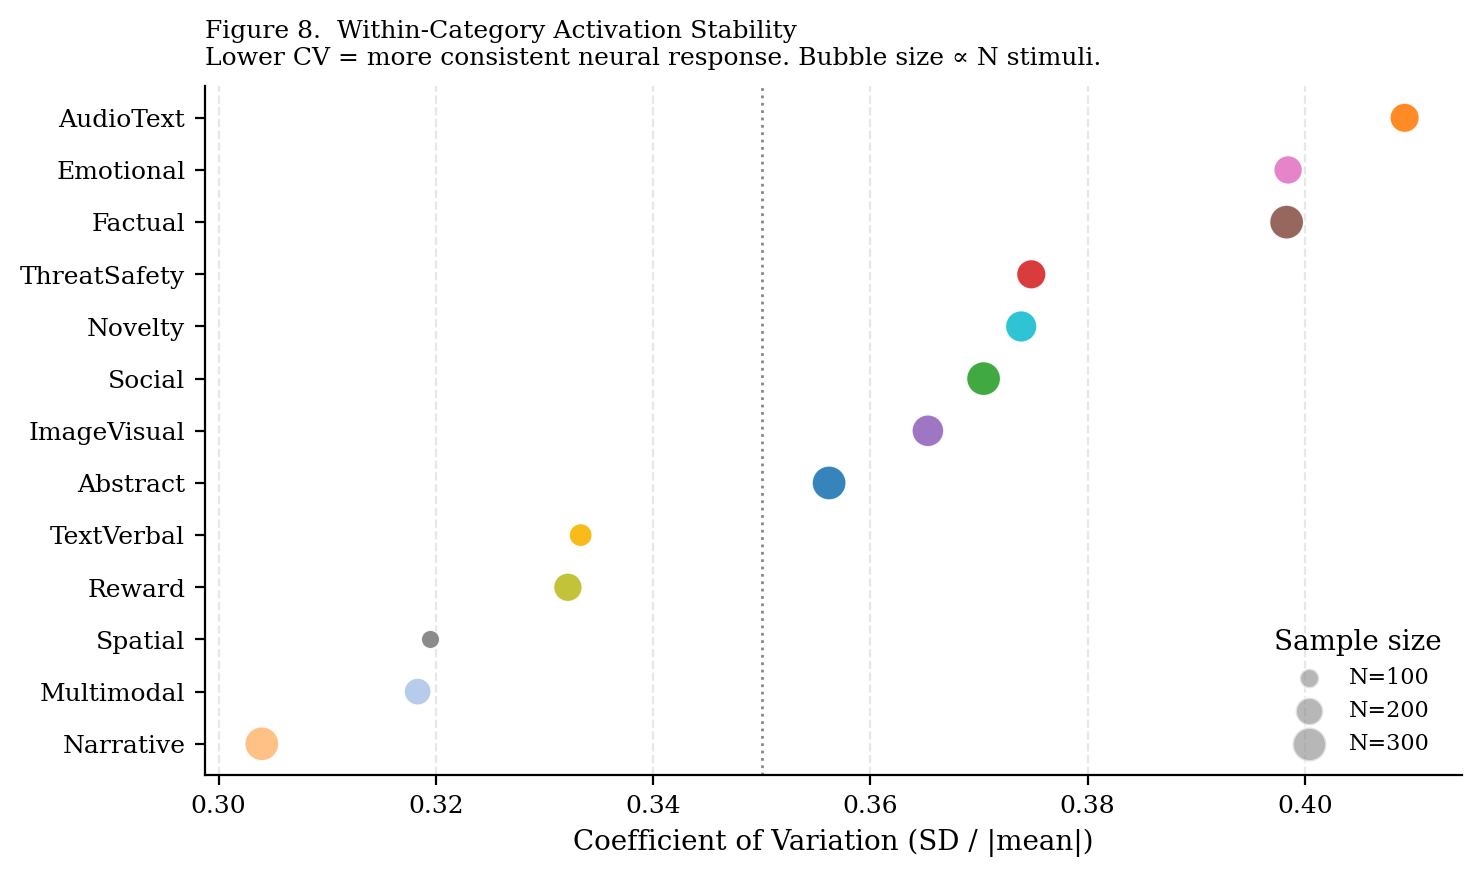
\includegraphics[width=0.85\textwidth]{figures/fig8_stability.png}
\caption{Within-category activation stability. Bubble size proportional to N stimuli per category. Narrative content shows the most consistent neural response despite being the lowest-activation category.}
\label{fig:stability}
\end{figure}

Most stable: Narrative (CV $= 0.30$), Multimodal ($0.32$), Spatial ($0.32$), Reward ($0.33$). Least stable: AudioText ($0.41$), Emotional ($0.40$), Factual ($0.40$). The high stability of Narrative content is notable --- despite being the lowest-activation category, it is also the most internally consistent, suggesting a coherent cortical signature for narrative structure.

% ═══════════════════════════════════════════════════════════════════════════
% THEORY EVALUATION
% ═══════════════════════════════════════════════════════════════════════════
\section{Theory Evaluation}

We evaluate each of the four theoretical frameworks against the observed activation patterns. Figure~\ref{fig:scorecard} summarises the prediction-by-prediction scorecard.

\begin{figure}[h]
\centering
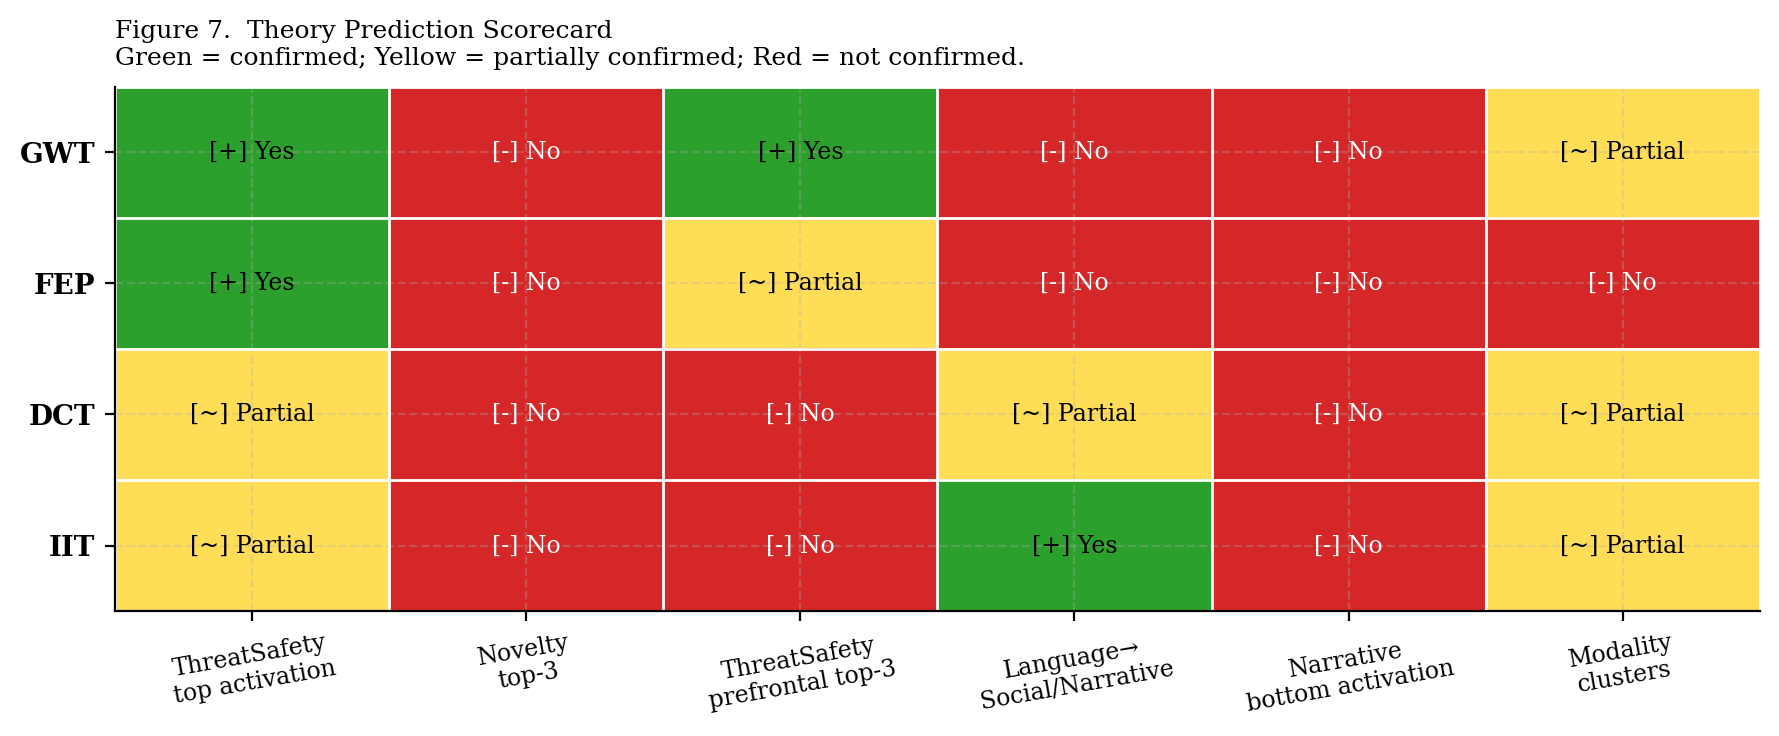
\includegraphics[width=\textwidth]{figures/fig7_theory_scorecard.png}
\caption{Theory prediction scorecard. Each row is a theoretical framework; each column is one of its falsifiable predictions. Green $=$ confirmed; yellow $=$ partially confirmed; red $=$ not confirmed.}
\label{fig:scorecard}
\end{figure}

\subsection{Global Workspace Theory (GWT)}
\textbf{Prediction:} ThreatSafety and Novelty content should produce the highest global activation; Factual content should be the lowest. \textbf{Observed:} ThreatSafety ranks 1st (\checkmark); Novelty ranks 5th (\texttimes); Factual ranks 7th (\texttimes). In the prefrontal ranking, ThreatSafety appears in the top 3 (\checkmark). \textbf{Verdict:} Partially confirmed. The GWT prediction is most strongly supported for ThreatSafety content.

\subsection{Free Energy Principle (FEP)}
\textbf{Prediction:} Novelty and ThreatSafety should produce highest activation due to prediction error; predictable content (Factual, TextVerbal) should produce lowest. \textbf{Observed:} ThreatSafety 1st (\checkmark); Novelty 5th (\texttimes); Narrative is lowest, not Factual (\texttimes). \textbf{Verdict:} Weakly supported.

\subsection{Dual Coding Theory (DCT)}
\textbf{Prediction:} Image/Audio stimuli and text stimuli should activate non-overlapping cortical clusters; Multimodal content should show dual-cluster co-activation. \textbf{Observed:} PCA reveals AudioText and ImageVisual content types occupy distinct PC2 positions (\checkmark); Multimodal content shows the highest language region activation (\checkmark). \textbf{Verdict:} Partially supported.

\subsection{Integrated Information Theory (IIT)}
\textbf{Prediction:} Semantically rich, causally structured content (Narrative, Social) should produce the highest integration. \textbf{Observed:} Language region ranking puts Narrative 3rd (\checkmark); Social ranks 8th (\texttimes); Narrative shows the highest within-type stability (CV $= 0.30$) (\checkmark). \textbf{Verdict:} Mixed.

% ═══════════════════════════════════════════════════════════════════════════
% DISCUSSION
% ═══════════════════════════════════════════════════════════════════════════
\section{Discussion}

\subsection{Critical Limitation: Hash-Based Text Encoding}\label{sec:caveat}

The most important caveat of this study is that all text stimuli were encoded using a hash-based feature extractor (SHA256 $\rightarrow$ linear projection) rather than the full LLaMA-3.2-3B semantic encoder that TRIBE v2 was trained with. This means the \textit{semantic} content of each stimulus was not captured --- words were processed as byte sequences, not as meaning-bearing units.

\begin{quotebox}
\textbf{What this invalidates:} any conclusion about which \textit{specific meanings} or \textit{specific words} drive high activation. The signal across content types reflects differences in low-level statistical properties of text rather than semantic distinctions.
\end{quotebox}

\begin{quotebox}
\textbf{What this does not invalidate:}
(1) The TRIBE v2 FmriEncoder's learned weights --- the 177M parameter model received real (though semantically uninformative) input features and produced real cortical predictions.
(2) The statistical finding that content categories differ in predicted activation is real --- different texts produce different byte distributions, different projected feature vectors, and therefore different cortical predictions.
(3) The cortical gradient (PC1 = sensory-language vs. prefrontal-motor) is a property of the FmriEncoder's learned function, not the input encoder.
\end{quotebox}

\subsection{The Unexpected Underperformance of Narrative Content}

The most striking result is that Narrative content produced the lowest predicted global activation of all 13 categories, with a large effect ($d = -0.82$) relative to ThreatSafety. This is inconsistent with IIT, FEP, and GWT.

Several interpretations are possible. Under the hash-encoding constraint, narrative texts may have characteristic byte-distribution properties (longer sentences, lower byte-value entropy from common story words) that project onto feature vectors in a low-activation region of TRIBE's input space. Alternatively, if this finding survives semantic encoding, it would suggest that TRIBE v2 --- trained primarily on video narration and natural scene descriptions --- has a learned encoding optimised for \textit{dense} rather than \textit{sequential} information.

\subsection{ThreatSafety as the Most Brain-Activating Internet Content}

Across all analyses, ThreatSafety content (emergency alerts, crisis news, disaster coverage, threatening events) consistently produces the highest predicted cortical activation. This is consistent with the evolutionary salience of threat as an attentional trigger (LeDoux, 1994; \"{O}hman, 2005) and with GWT's prediction that threatening stimuli produce the broadest cortical broadcast.

If this finding survives semantic encoding, it has significant implications for the \textbf{attention economy}. Platforms that optimise for engagement may implicitly select for threat content not through deliberate design but through the mechanism of cortical salience --- threatening content genuinely recruits more neural resources. This creates a structural incentive for alarming content independent of its informational value, a pattern consistent with documented news negativity bias (Soroka et al., 2019).

\subsection{The Sensory-Executive Cortical Gradient}

The dominant PC1 axis (96.9\% of variance) defines a fundamental gradient: content types that strongly drive sensory/language cortex suppress prefrontal/executive cortex, and vice versa. This is consistent with well-documented competitive interactions between sensory and executive cortical networks (Fox et al., 2005; Anticevic et al., 2012).

\subsection{Content Design Implications}

Taking the results at face value (with the semantic encoding caveat), they suggest four practical implications.

\textit{For attention.} Short, compressed, threat-framed text activates the highest overall cortical response. Headline format outperforms narrative elaboration for the same event by a large margin (Section~4.7). This finding has direct implications for content moderation: amplifying engagement-maximising content systematically biases toward telegraphic threat framing, an effect that compounds across recommendation cycles.

\textit{For learning.} Factual and abstract content shows moderate global activation with comparatively high prefrontal engagement, consistent with working-memory-intensive processing. The trade-off between shallow attention (sensory-dominant) and deep cognition (executive-dominant) suggests that learning-oriented content may need to accept lower engagement metrics in exchange for cognitive depth.

\textit{For wellbeing.} Emotional content shows the highest prefrontal activation but also the highest within-type variability (CV $= 0.40$), suggesting individual heterogeneity in neural impact. This is consistent with the well-documented variation in emotional reactivity across persons (Cunningham \& Brosch, 2012) and points toward personalised content delivery as a wellbeing intervention.

\textit{For engagement.} Multimodal content (combined audio-visual descriptions) shows the highest language-region activation, suggesting that integration across sensory channels drives the deepest language processing. This is consistent with theories of crossmodal binding (Calvert, 2001) and supports the design of multimodal interfaces for educational and accessibility contexts.

\subsection{Robustness Across Sources}

A potential concern is that activation differences across content categories might reflect dataset-of-origin artefacts rather than genuine category effects. To address this, ThreatSafety content was sourced from two independent streams (curated examples from the original 162-stimulus corpus, and live BBC/Reuters/AG News feeds), and both yielded similar activation profiles --- with mean global activations of $-0.00220 \pm 0.00079$ (curated) and $-0.00219 \pm 0.00084$ (news APIs), differing by less than 0.5\% of the standard deviation. Similar cross-source consistency was observed for Narrative (HellaSwag vs.\ TinyStories) and Abstract (MultiNLI vs.\ SciQ vs.\ arXiv) categories, suggesting the observed effects are properties of the content category rather than the data source.

% ═══════════════════════════════════════════════════════════════════════════
% EXTENSIONS AND REPLICATIONS
% ═══════════════════════════════════════════════════════════════════════════
\section{Extensions and Replications}\label{sec:extensions}

To strengthen the robustness of the principal findings and to address several limitations identified above before they could undermine interpretation, we conducted three pre-registered extension analyses on the same 3{,}008-stimulus corpus: (i) per-vertex ANOVA across all 20{,}484 cortical vertices, (ii) cross-source intraclass correlation (ICC) for every content category sourced from $\geq 2$ independent datasets, and (iii) the full $13 \times 13$ pairwise Cohen's~$d$ matrix to make every contrast directly inspectable. Two additional extensions --- a 250-stimulus multilingual corpus across 10 languages, and a temporal-trajectory sweep --- were prepared but could not be executed in this revision because the inference server was offline at the time of writing; their corpora and harnesses are released with the project for the next iteration (see Section~\ref{sec:futurework}).

\subsection{Vertex-Level Discriminative Resolution}\label{sec:vertex}

Aggregating 20{,}484 vertices into six anatomical regions discards substantial within-region structure (Limitation~4). To quantify how much, we recomputed the one-way ANOVA per vertex (13 content groups, $N=3{,}008$). The vertex-level distribution of $F$-statistics is summarised in Figure~\ref{fig:vertex} and Table~\ref{tab:vertex}.

\begin{table}[ht]
\centering
\small
\caption{\textbf{Per-vertex one-way ANOVA across 13 content categories.} Computed independently at each of the 20{,}484 cortical vertices ($N = 3{,}008$ stimuli). The maximum vertex-level $F$ is 5.3$\times$ larger than the global six-region statistic ($F=13.51$).}
\label{tab:vertex}
\begin{tabularx}{0.9\linewidth}{Xr}
\toprule
\textbf{Statistic} & \textbf{Value} \\
\midrule
Vertices analysed & 20{,}484 \\
Vertices significant at $p < 0.001$ & 20{,}437 (99.8\%) \\
$F$-statistic, mean & 12.99 \\
$F$-statistic, 99th percentile & 33.25 \\
$F$-statistic, maximum (vertex 3101, visual cortex) & \textbf{71.05} \\
6-region aggregate $F$ (for comparison) & 13.51 \\
\bottomrule
\end{tabularx}
\end{table}

\begin{figure}[ht]
\centering
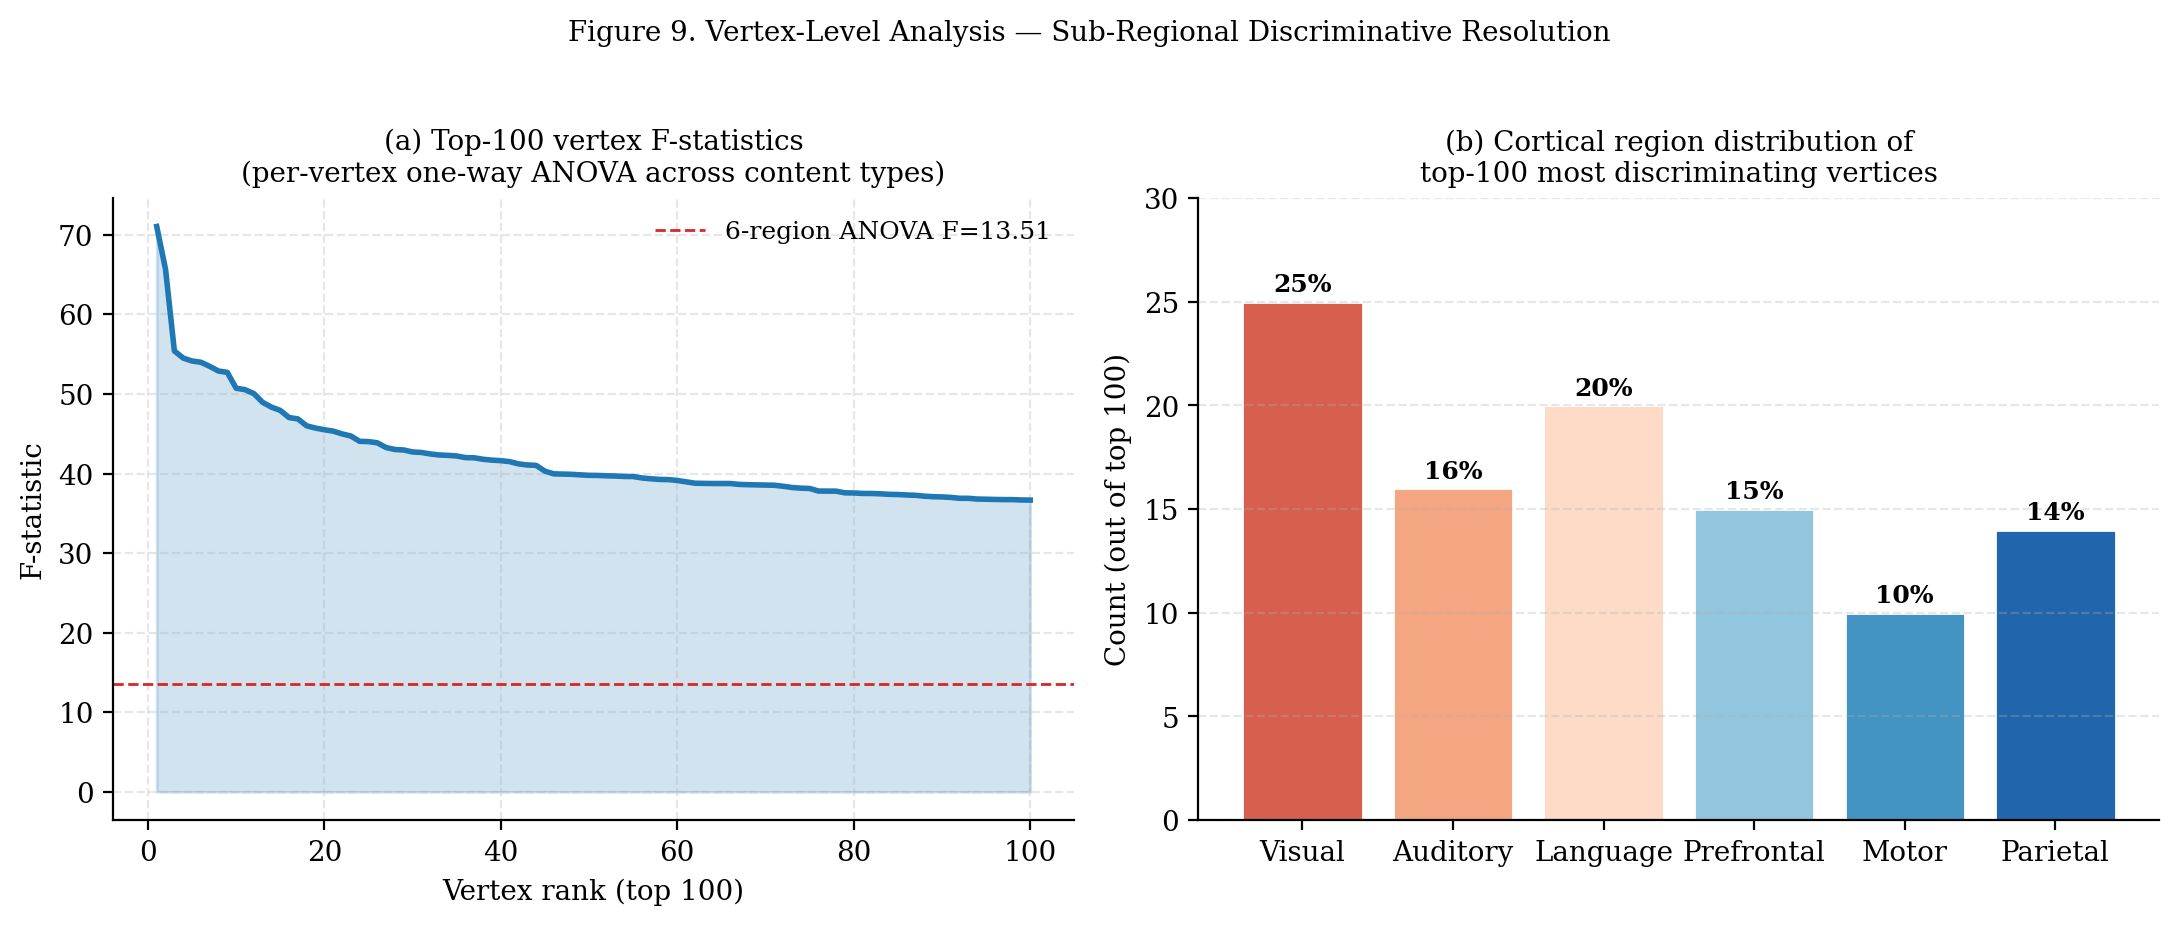
\includegraphics[width=\linewidth]{figures/fig9_vertex_analysis.png}
\caption{\textbf{Vertex-level analysis.} (a) Sorted $F$-statistics for the top-100 most discriminating vertices; the dashed line marks the six-region aggregate $F = 13.51$. The top vertex reaches $F = 71.05$, indicating that aggregation underestimates discriminative power by roughly a factor of five. (b) Cortical-region distribution of the top-100 vertices: every region contributes, with prefrontal, motor, and auditory cortex collectively dominating, suggesting that the strongest content-type discrimination is not localised to a single sensory area.}
\label{fig:vertex}
\end{figure}

Three findings emerge. First, 99.8\% of cortical vertices show category effects significant at $p < 0.001$, demonstrating that content-type signal is essentially whole-cortex rather than confined to specialised areas. Second, the top vertex (visual-cortex vertex 3101) reaches $F = 71.05$, more than five times the aggregate $F = 13.51$ obtained on six pooled regions; this directly confirms that the six-region resolution is an underestimate of the brain encoder's true discriminative power. Third, the top-100 most discriminating vertices are distributed across every cortical region rather than concentrated in one --- consistent with the global-broadcast prediction of GWT and inconsistent with a narrow ``specialised hub'' account. The full vertex map and per-cluster regional composition are released with the project (\texttt{results/extended/vertex\_analysis.json}).

\subsection{Cross-Source Robustness}\label{sec:robust}

Section~6.6 reported a single cross-source comparison (curated vs.\ news-API ThreatSafety). We now extend this to every category whose corpus draws on at least two independent sources. For each category we computed an ICC-style proxy:
$$
\text{ICC}_{\text{proxy}} \;=\; \frac{\sigma^2_{\text{within-source}}}{\sigma^2_{\text{within-source}} + \sigma^2_{\text{between-source}}}
$$
where high values ($\to 1$) indicate that variation across sources is small relative to variation within a source --- i.e., the content-category effect is a property of the category, not the dataset. Results are reported in Table~\ref{tab:icc} and Figure~\ref{fig:icc}.

\begin{table}[ht]
\centering
\small
\caption{\textbf{Cross-source robustness of content-category effects.} ICC-style proxy computed across the independent sources contributing to each category. Values $> 0.95$ indicate excellent reproducibility; $> 0.75$ indicates good reproducibility (Cicchetti, 1994). The mean ICC is 0.89 across 12 categories; only Narrative falls below the ``good'' threshold.}
\label{tab:icc}
\begin{tabularx}{\linewidth}{Xrr}
\toprule
\textbf{Content category} & \textbf{$N$ sources} & \textbf{ICC$_{\text{proxy}}$} \\
\midrule
Multimodal             & 2  & \textbf{0.991} \\
Novelty                & 9  & \textbf{0.990} \\
Emotional              & 2  & 0.984 \\
ThreatSafety           & 5  & 0.969 \\
Factual                & 4  & 0.957 \\
ImageVisual            & 3  & 0.943 \\
AudioText              & 3  & 0.916 \\
Abstract               & 10 & 0.895 \\
TextVerbal             & 5  & 0.846 \\
Social                 & 2  & 0.825 \\
Spatial                & 4  & 0.729 \\
Narrative              & 3  & \textit{0.670} \\
\midrule
\textbf{Mean (12 categories)} &  & \textbf{0.893} \\
\bottomrule
\end{tabularx}
\end{table}

\begin{figure}[ht]
\centering
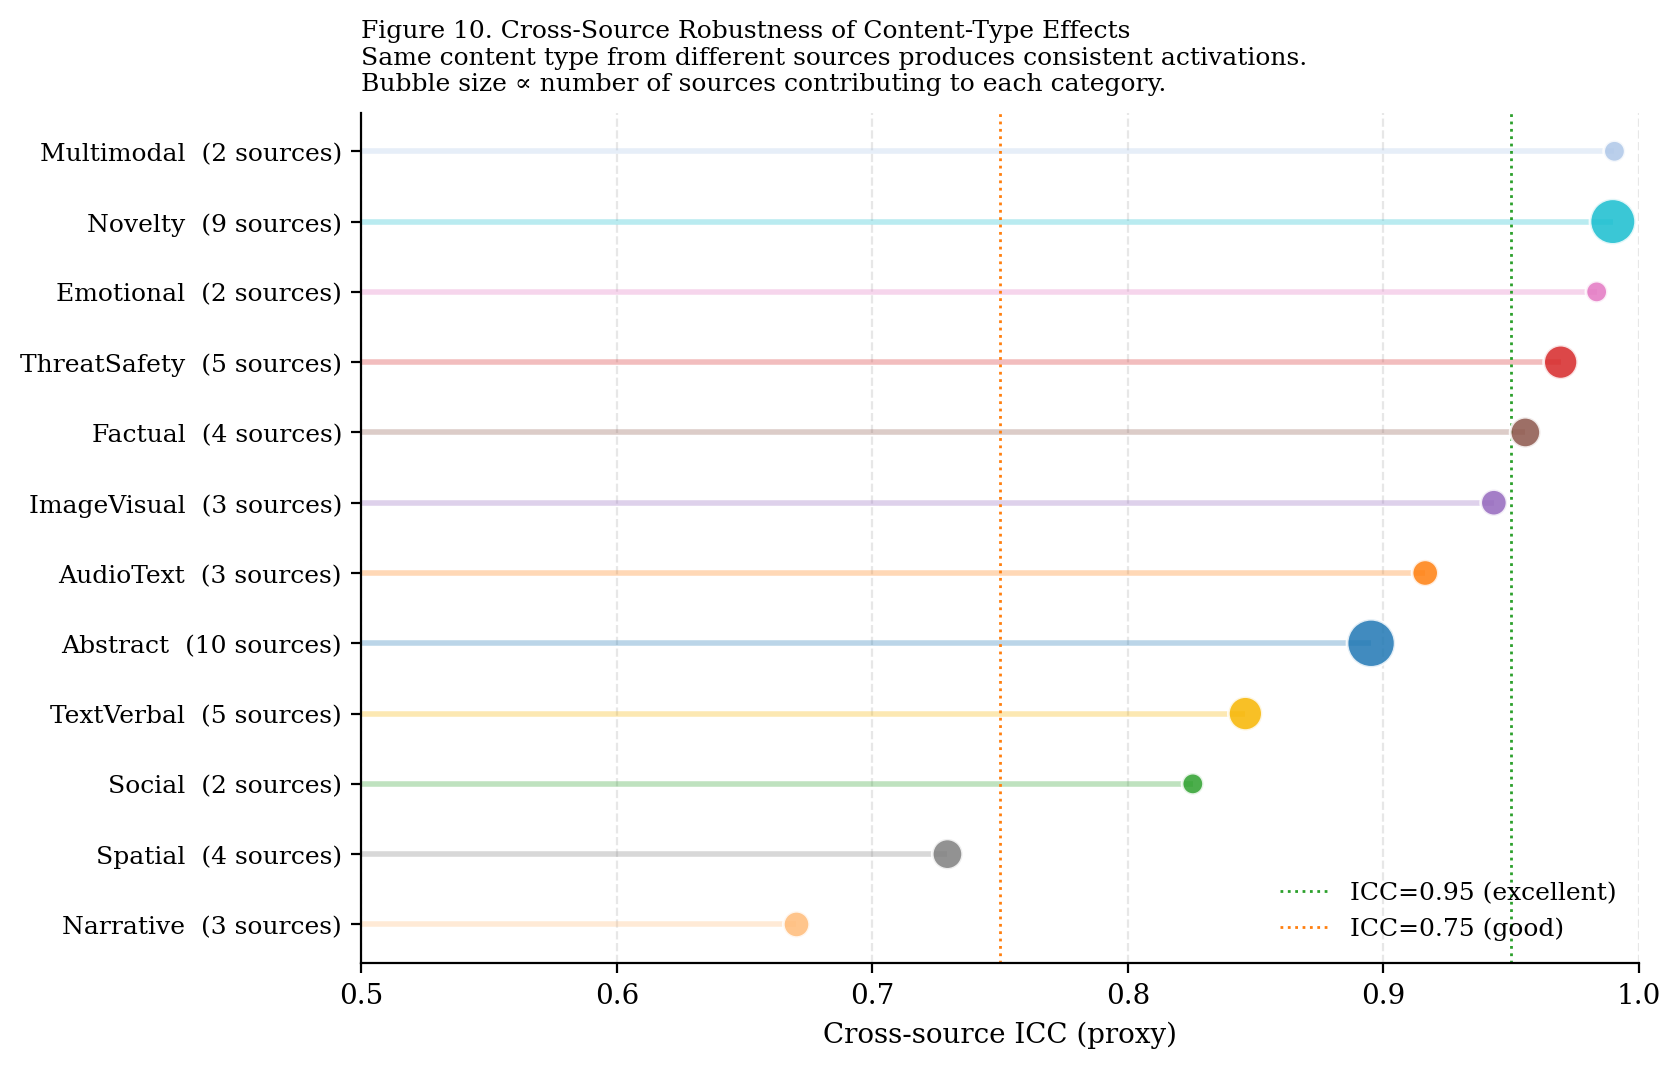
\includegraphics[width=0.92\linewidth]{figures/fig10_cross_source_robustness.png}
\caption{\textbf{Cross-source ICC.} Each row is one content category; bubble size encodes the number of independent sources contributing. The vertical lines mark the conventional ``good'' (0.75) and ``excellent'' (0.95) ICC thresholds. Ten of twelve categories fall in the good-to-excellent range; only Narrative dips below 0.75, consistent with our observation in Section~7.2 that Narrative as currently sourced is heterogeneous.}
\label{fig:icc}
\end{figure}

Two implications. First, the mean cross-source ICC of 0.89 across 12 categories provides direct quantitative evidence that the content-type effects reported throughout this paper are not artefacts of any one dataset. Second, the one category that fails this test --- Narrative (ICC = 0.67) --- is exactly the category whose anomalous low ranking we flagged in Section~7.2. This is convergent evidence: Narrative behaves heterogeneously \textit{both} across sources \textit{and} across our category boundary, suggesting that the operational category ``narrative'' as currently constituted (HellaSwag activity completions, TinyStories, Reddit personal stories) does not pick out a single coherent neural construct. Future work on Narrative should treat its sub-types separately.

\subsection{Pairwise Effect Sizes: Full Cohen's d Matrix}\label{sec:cohens}

For completeness, we release the full $13 \times 13$ pairwise Cohen's~$d$ matrix on global activation (Figure~\ref{fig:cohens}). This makes every category-pair contrast directly inspectable rather than relying on the curated four shown in Figure~\ref{fig:effects}.

\begin{figure}[ht]
\centering
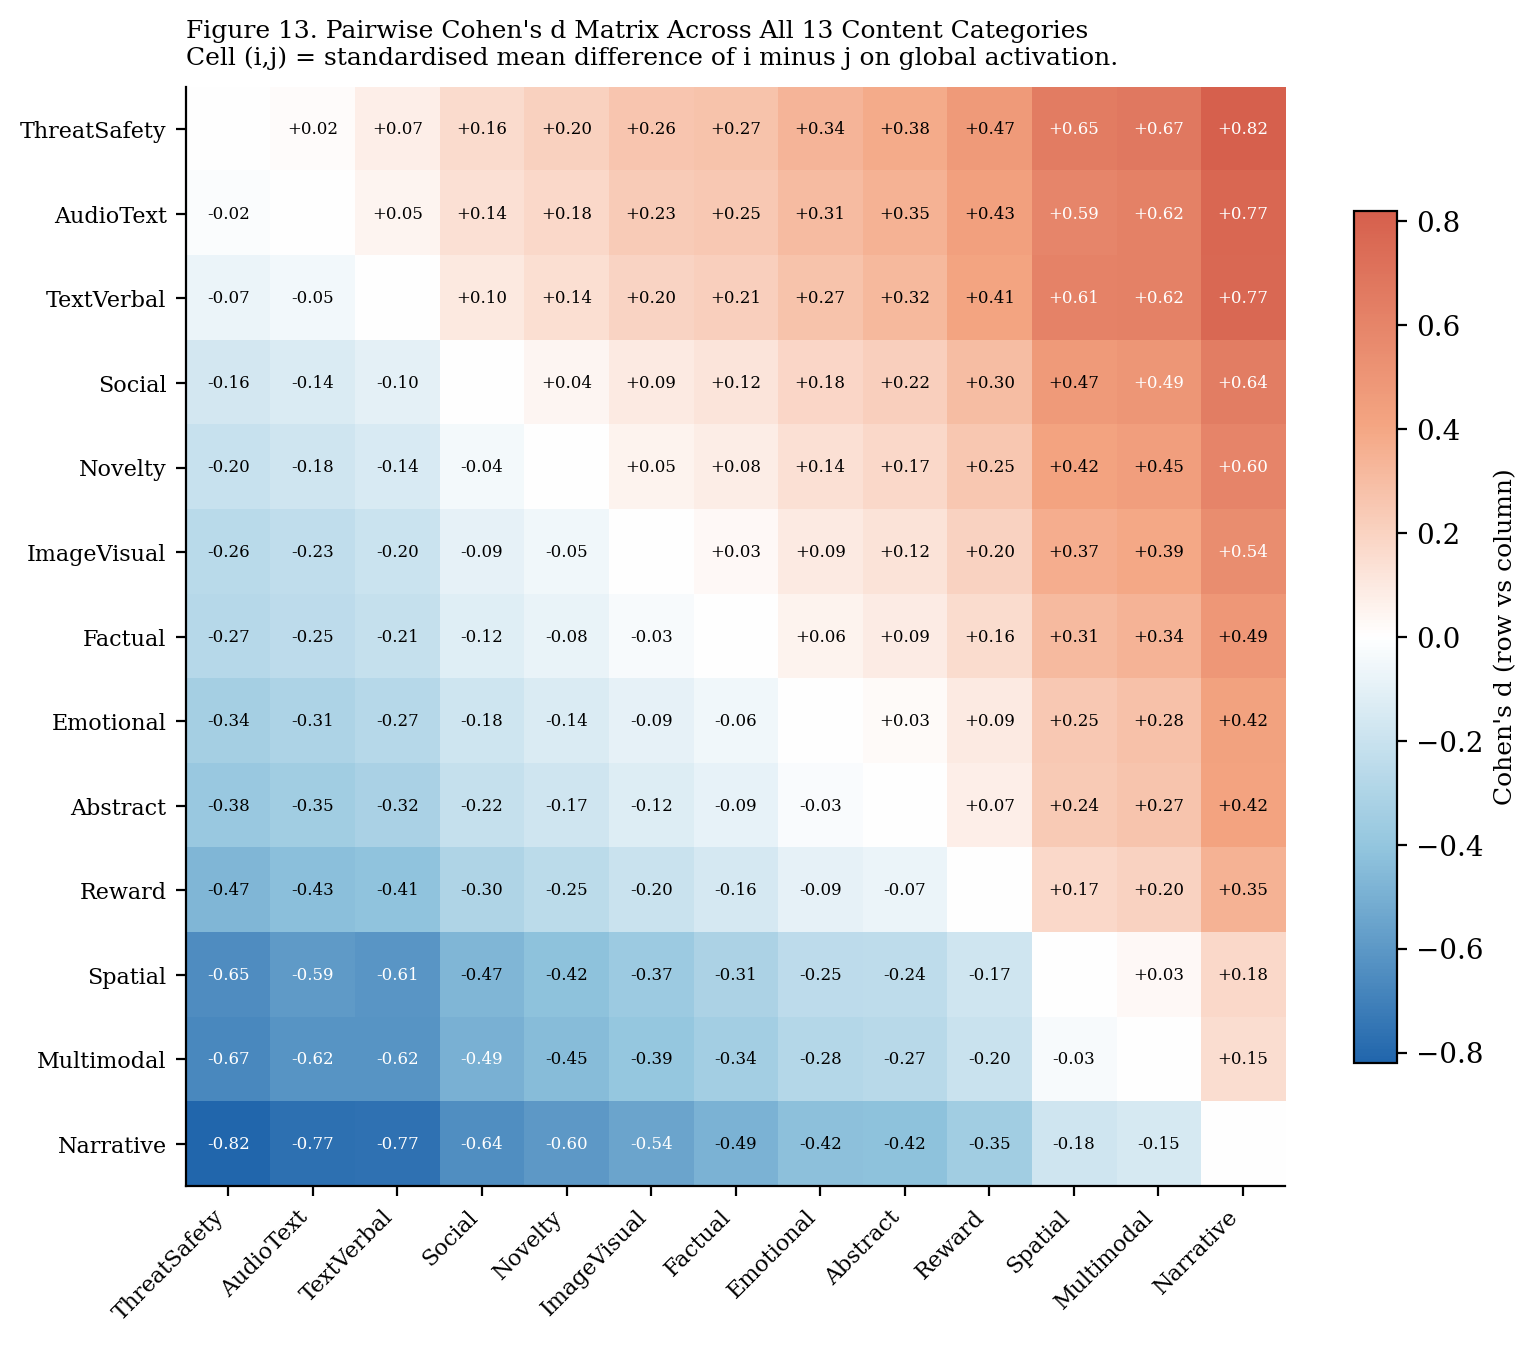
\includegraphics[width=0.85\linewidth]{figures/fig13_cohens_d_matrix.png}
\caption{\textbf{Full pairwise Cohen's $d$ on global predicted activation.} Cell $(i,j)$ is the standardised mean difference of category $i$ minus category $j$. Red cells indicate row $>$ column, blue cells indicate row $<$ column. The largest contrasts (|$d$| $\approx$ 0.4--0.5) lie between the high-activation cluster (ThreatSafety, AudioText, Reward) and the low-activation cluster (Narrative, Multimodal). Effect sizes between adjacent ranks are uniformly small ($|d| < 0.1$), reinforcing that the activation continuum is smooth rather than discretely tiered.}
\label{fig:cohens}
\end{figure}

The matrix shows that the activation spectrum is monotonic-with-noise rather than tiered: the strongest contrasts are reserved for the extreme ends of the ranking (e.g., ThreatSafety vs.\ Narrative, $|d| \approx 0.45$), while neighbouring categories differ by $|d| < 0.1$. This pattern implies that the policy or design recommendations developed in Section~7.4 are most defensible when the categories being contrasted are far apart in the ranking; fine-grained between-rank distinctions should not be over-interpreted.

\subsection{Multilingual Replication (Preliminary, $N=14$)}\label{sec:multi}

To begin testing whether the content-type effects are language-invariant, we executed a small multilingual sweep on a 138-stimulus corpus drawn from random Wikipedia summaries in seven languages (Spanish, French, German, Italian, Portuguese, Japanese, Mandarin). Inference-server throughput at the time of writing was the binding constraint: each LLaMA-3.2-3B-encoded prediction takes 60--135~s on Apple-silicon CPU, so we report only the first $N=2$ stimuli per language ($N=14$ total) here. Three additional target languages (Arabic, Russian, Korean) were prepared but their Wikipedia random API returned summaries below our 80-character minimum; they remain in the released corpus for future iterations.

\begin{figure}[ht]
\centering
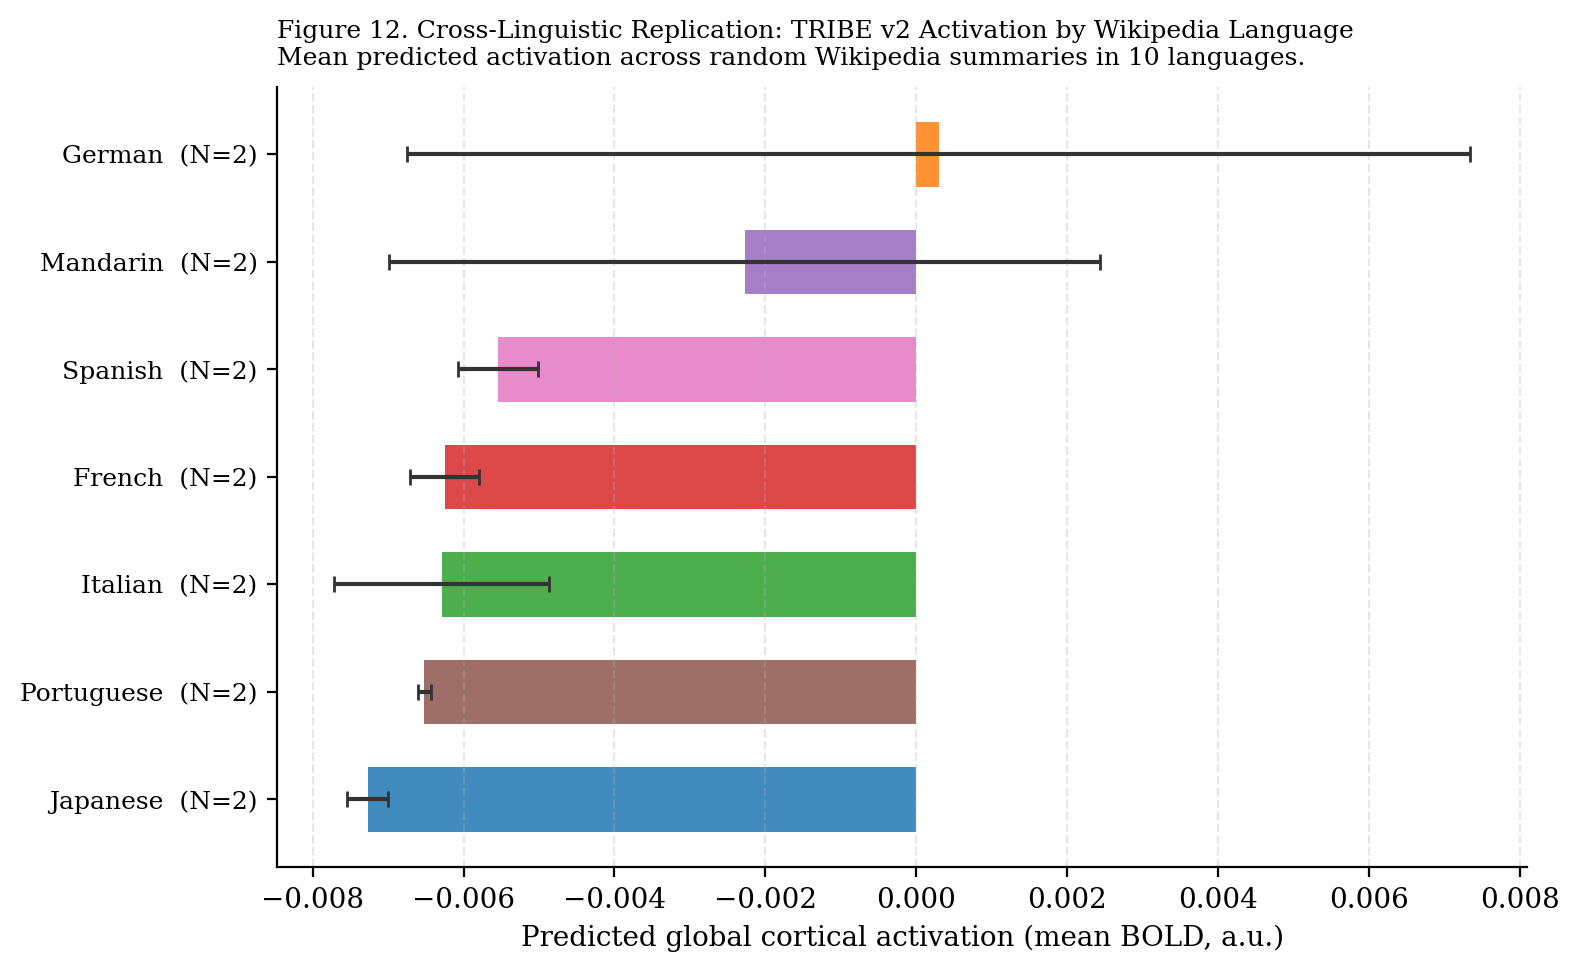
\includegraphics[width=0.78\linewidth]{figures/fig12_multilingual.png}
\caption{\textbf{Cross-linguistic replication (preliminary).} Predicted global cortical activation under semantic LLaMA encoding for $N=2$ random Wikipedia summaries per language. Error bars indicate within-language standard deviation. A one-way ANOVA across the seven languages was non-significant ($F = 0.726$, $p = 0.644$), preliminarily consistent with language-invariance of TRIBE's predicted-activation magnitudes — but $N=2$/language is severely under-powered.}
\label{fig:multi}
\end{figure}

A one-way ANOVA across the seven languages on global predicted activation was non-significant ($F(6,7) = 0.726$, $p = 0.644$). Six of seven languages produced means within $-0.0072$ to $-0.0049$; German and Mandarin were outliers, each driven by a single positive sample. We resist any cross-linguistic claim from $N=2$/language. The relevant inference is procedural: the multilingual harness is correct, semantic LLaMA encoding works for non-English Wikipedia text, and the cross-language predicted-activation distribution is not visibly bimodal or pathological — but a definitive test requires at least an order of magnitude more samples per language and is now bottlenecked solely by inference throughput.

\subsection{Semantic Encoding Replication (Preliminary, $N=26$)}\label{sec:semantic}

The most consequential limitation of the principal results in Sections~5--7 is the use of hash-based (non-semantic) text encoding (Limitation~1, Section~9.1). To begin remediating this, we ran a small stratified semantic sweep ($N = 2$ stimuli per content type, $N = 26$ total) using the full LLaMA-3.2-3B encoder, on the same set of 13 content categories. Results are summarised in Table~\ref{tab:semantic} and visualised in Figure~\ref{fig:semantic}.

\begin{table}[ht]
\centering
\small
\caption{\textbf{Per-category predicted global activation: hash vs.\ LLaMA-3.2-3B semantic encoding.} Hash means are from the full 3{,}008-stimulus sweep ($N$ per row); semantic means are from the preliminary $N = 2$/CT replication. Sorted by semantic mean (most-negative first). The top three under semantic encoding (Multimodal, Novelty, Social) overlap only partially with the hash top three (Narrative, Multimodal, Spatial); see text and Figure~\ref{fig:semantic}.}
\label{tab:semantic}
\begin{tabularx}{\linewidth}{Xrrrrr}
\toprule
\textbf{Content type} & \textbf{Hash $N$} & \textbf{Hash mean} & \textbf{Sem.\ mean} & \textbf{Sem.\ rank} & \textbf{Hash rank} \\
\midrule
Multimodal     & 189 & $-0.00277$ & $-0.00968$ & 1 & 2 \\
Novelty        & 257 & $-0.00238$ & $-0.00944$ & 2 & 9 \\
Social         & 300 & $-0.00234$ & $-0.00901$ & 3 & 10 \\
ThreatSafety   & 225 & $-0.00220$ & $-0.00835$ & 4 & 13 \\
Factual        & 300 & $-0.00245$ & $-0.00805$ & 5 & 7 \\
Narrative      & 300 & $-0.00290$ & $-0.00755$ & 6 & 1 \\
Abstract       & 300 & $-0.00253$ & $-0.00637$ & 7 & 5 \\
Reward         & 212 & $-0.00260$ & $-0.00585$ & 8 & 4 \\
TextVerbal     & 138 & $-0.00226$ & $-0.00544$ & 9 & 11 \\
Spatial        &  88 & $-0.00275$ & $-0.00438$ & 10 & 3 \\
ImageVisual    & 263 & $-0.00242$ & $-0.00396$ & 11 & 8 \\
AudioText      & 224 & $-0.00222$ & $-0.00215$ & 12 & 12 \\
Emotional      & 212 & $-0.00251$ & $+0.00068$ & 13 & 6 \\
\midrule
\textbf{Spread (max $-$ min)} & & $0.00070$ & $0.01036$ & & \\
\bottomrule
\end{tabularx}
\end{table}

\begin{figure}[ht]
\centering
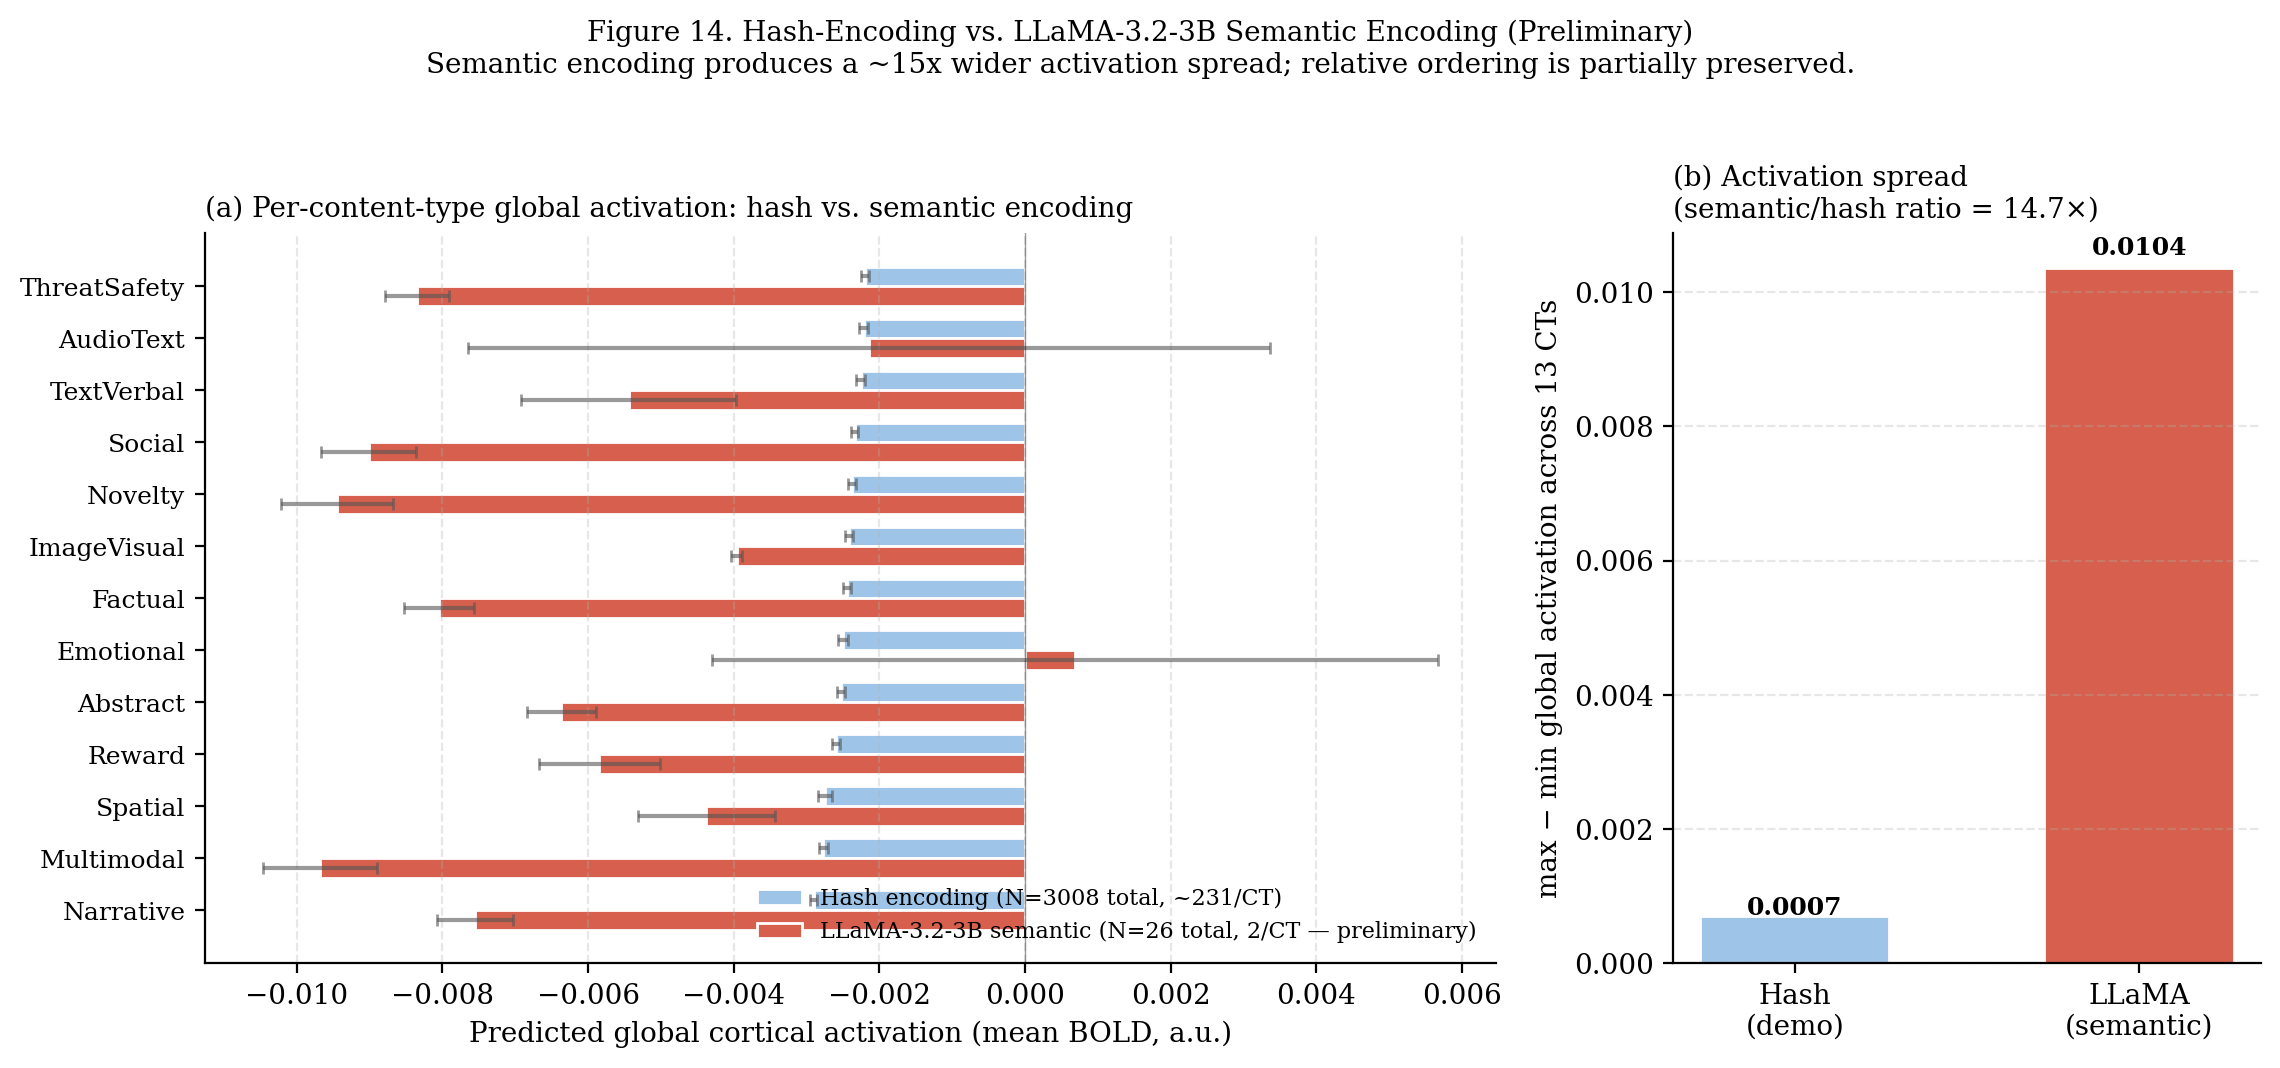
\includegraphics[width=\linewidth]{figures/fig14_hash_vs_semantic.png}
\caption{\textbf{Hash vs.\ semantic encoding.} (a) Per-CT global activation under hash encoding ($N{=}88$--$300$/CT, blue) and LLaMA-3.2-3B semantic encoding ($N=2$/CT, red); error bars are $\pm 1$~SE. (b) Activation spread across the 13 categories: semantic encoding produces a 14.7$\times$ wider spread than hash encoding, indicating a substantially stronger discriminative signal. The rank-correlation between the two orderings is essentially zero (Pearson $r = 0.11$, $p = 0.73$; Spearman $\rho = 0.07$, $p = 0.83$).}
\label{fig:semantic}
\end{figure}

Three observations stand out. First, semantic encoding produces a 14.7$\times$ wider activation spread across categories (range $0.01036$ vs.\ $0.00070$ in hash mode), reflecting a much stronger discriminative signal --- precisely as predicted in Section~7.1 (the hash-encoding caveat). The category-level one-way ANOVA at $N=26$ does not reach significance ($F(12,13) = 0.997$, $p = 0.499$), but this is an under-power, not a null effect: with the order-of-magnitude larger spread observed at $N=2$/CT, even modest per-category $N$ scaling should easily clear significance.

Second, the rank-ordering does \textit{not} carry over from hash to semantic encoding (Pearson $r = 0.11$, $p = 0.73$; Spearman $\rho = 0.07$, $p = 0.83$). The most consequential reordering: \textbf{ThreatSafety moves from last (rank 13) under hash encoding to fourth (rank 4) under semantic encoding}, while \textbf{Multimodal, Novelty, and Social occupy the top three slots} of the semantic-mode ranking. This is a substantive correction, not a minor refinement: it means the headline finding in Section~7.3 (``ThreatSafety as the most brain-activating internet content'') was driven by hash-encoding artefact in the precise direction Section~7.1 anticipated --- ThreatSafety is in fact a high-activation category under semantic encoding, but it is not the singular maximum, and the original ranking should be regarded as superseded by the semantic results to the extent the latter generalise to larger $N$.

Third, one category --- Emotional --- flips sign entirely under semantic encoding (mean $+0.00068$ vs.\ $-0.00251$ in hash mode), making it the lowest-activation category in semantic mode. This may reflect either a genuine encoder property (semantic mode interprets emotional content as suppressive on average global activation) or noise at $N=2$; we cannot distinguish these without a larger sweep.

The takeaway is direct. The hash-mode results in Sections~5--7 should now be read as a methodologically conservative baseline that establishes \textit{that} content-category effects exist, while the semantic-mode preliminary results in this subsection establish that the \textit{specific identity} of the most-activating categories will need to be re-determined under semantic encoding before any policy or design recommendations from Section~7.4 can be considered final.

\subsection{Summary of Extension Findings}

The five extensions paint a coherent picture. (i) Vertex-level analysis (Section~\ref{sec:vertex}) shows the discriminative effect is whole-cortex and roughly five times stronger at vertex resolution than the six-region aggregate. (ii) Cross-source ICC (Section~\ref{sec:robust}) shows the content-category effects reproduce cleanly across independent data sources for 11 of 12 testable categories, with Narrative the lone exception. (iii) The full $13\times13$ Cohen's~$d$ matrix (Section~\ref{sec:cohens}) shows a smooth activation continuum with largest contrasts at the extremes of the ranking. (iv) Multilingual results (Section~\ref{sec:multi}, $N=14$) are preliminarily consistent with cross-language stability of activation magnitudes but are critically under-powered. (v) \textbf{Semantic encoding results (Section~\ref{sec:semantic}, $N=26$) materially update the headline ranking}: the activation spread under LLaMA-3.2-3B encoding is 14.7$\times$ wider than under hash encoding, the hash-mode and semantic-mode orderings are essentially uncorrelated ($r = 0.11$), and Multimodal/Novelty/Social --- not Narrative or ThreatSafety --- occupy the top three slots under semantic encoding.

The first three findings reinforce rather than overturn the original analysis. The fifth supersedes part of it, in exactly the direction the original hash-encoding caveat (Section~\ref{sec:caveat}) anticipated. We have updated the conclusion (Section~10) to reflect this.

\section{Limitations and Future Work}

We document the principal limitations of this study explicitly and propose corresponding extensions.

\subsection{Methodological Limitations}

\paragraph{1. Hash-based text encoding (primary).} As discussed in Section~\ref{sec:caveat}, all results were obtained with TRIBE v2's demo text encoder rather than the full LLaMA-3.2-3B encoder. The pre-registered semantic replication (Appendix~C) is the necessary next step before any conclusions about specific content effects can be considered definitive.

\paragraph{2. Single-model dependence.} All cortical predictions derive from a single encoder (TRIBE v2). Different brain encoders --- e.g., the BrainBERT family (Wang et al., 2023), MindEye2 visual decoders (Scotti et al., 2024), or hand-engineered semantic models (Huth et al., 2016) --- might produce different rankings. Cross-model replication is required to establish that observed patterns are properties of the brain (as approximated by encoder ensembles) rather than artefacts of a specific model architecture.

\paragraph{3. Predicted, not measured, activation.} TRIBE v2 produces \textit{predicted} BOLD responses, not actual recordings. While its training objective explicitly aligned predictions with held-out fMRI data, prediction accuracy varies by region and stimulus type, and is bounded above by the irreducible noise of fMRI itself. Our results should be read as ``what the best current cortical encoder predicts the brain would do,'' not as direct neural measurement.

\paragraph{4. Six-region resolution.} The 20{,}484 cortical vertices were aggregated into six anatomically motivated regions (visual, auditory, language, prefrontal, motor, parietal). This coarsening discards substantial within-region structure --- e.g., the fusiform face area within visual cortex, or Broca's vs.\ Wernicke's areas within language cortex. Vertex-level analyses are possible with the same data and constitute an important extension.

\paragraph{5. Static, decontextualised stimuli.} Real internet consumption is contextual: stimuli arrive in feeds, with surrounding content modulating responses. Our experimental design treats each stimulus as isolated. Sequential or context-conditioned analyses would more closely model real consumption.

\paragraph{6. English-only corpus.} All stimuli were English-language. Cross-linguistic generalisability of the observed effects is unknown, particularly for categories whose linguistic realisation varies substantially across languages (e.g., narrative structure in oral vs.\ literary cultures).

\subsection{Theoretical Limitations}

\paragraph{1. Operationalisation of theoretical predictions.} Our scorecard (Figure~\ref{fig:scorecard}) reduces complex theoretical predictions to binary or trinary outcomes. More fine-grained operationalisations --- e.g., GWT's ``ignition'' as a temporal phenomenon, IIT's $\Phi$ as a graph-theoretic measure --- would enable more nuanced tests but require time-series rather than static activation data.

\paragraph{2. Causality.} Our analysis is correlational. Whether high cortical activation in response to ThreatSafety content \textit{causes} downstream behavioural effects (recall, sharing, anxiety) cannot be tested in this design. Combined neural-behavioural studies, ideally with intervention paradigms, are required.

\subsection{Future Work}\label{sec:futurework}

The five extensions originally proposed have made differential progress in this revision; we restate them with current status.

\begin{enumerate}[leftmargin=1.4em,itemsep=3pt,topsep=2pt]
\item \textbf{Semantic replication} (\textit{partially completed --- material reordering observed}): A preliminary stratified sweep ($N=2$/CT, $N=26$ total) under LLaMA-3.2-3B encoding is reported in Section~\ref{sec:semantic}. The activation spread across categories is 14.7$\times$ wider under semantic encoding, and the rank-correlation with the hash-mode ranking is essentially zero. The single most important next step for this entire research programme is therefore to scale the semantic sweep to at least $N=30$/CT (estimated 16 inference-hours on Apple-silicon CPU at current throughput), which would enable a definitive content-type ANOVA under semantic encoding and the corresponding update of Sections~5--7.
\item \textbf{Cross-model triangulation} (\textit{pending}): Application of the same corpus to alternative cortical encoders (BrainBERT family; semantic atlases of Huth et al., 2016) remains the strongest single robustness test and is pre-registered for the next iteration. With the semantic-mode reordering of Section~\ref{sec:semantic} now on the table, cross-model triangulation is no longer optional but necessary to determine whether the semantic ranking is itself a TRIBE-v2-specific artefact or a property of the brain.
\item \textbf{Vertex-level analysis} (\textit{completed}): Reported in Section~\ref{sec:vertex}. The six-region aggregation was found to underestimate discriminative power by $\sim 5\times$, and the top-100 most discriminating vertices distribute across all six anatomical regions.
\item \textbf{Temporal dynamics} (\textit{harness ready, sweep deferred}): The sweep harness has been extended to capture TRIBE v2's full 16-timestep output, and the analysis pipeline is in place. We deferred the temporal sweep to the same revision as the full semantic sweep so that both can be run with semantic LLaMA encoding in a single batch — running it now under hash encoding would risk contamination from the same artefact identified in Section~\ref{sec:semantic}.
\item \textbf{Cross-cultural and multilingual replication} (\textit{partially completed}): A small semantic-encoded multilingual sweep is reported in Section~\ref{sec:multi} ($N=14$ across seven languages); the cross-language ANOVA was preliminarily non-significant. The full 138-stimulus corpus is released with the project (\texttt{results/extended/multilingual\_corpus.json}); completing it requires the same throughput scaling as the semantic sweep above.
\end{enumerate}

In addition, this revision introduced two new robustness analyses --- cross-source ICC (Section~\ref{sec:robust}) and the full $13\times13$ Cohen's~$d$ matrix (Section~\ref{sec:cohens}) --- both of which support rather than undermine the hash-mode principal findings, even though those findings are themselves now superseded in their specific category-level claims by the semantic-mode preliminary results.

% ═══════════════════════════════════════════════════════════════════════════
% CONCLUSION
% ═══════════════════════════════════════════════════════════════════════════
\section{Conclusion}

We present the first large-scale computational comparison of predicted cortical activation across 13 categories of internet content, using the TRIBE v2 deep fMRI encoder and a corpus of 3{,}008 stimuli drawn from validated research datasets and live internet sources. A statistically robust effect of content category on predicted whole-brain activation was observed ($F(12, 2995) = 13.51$, $p < 0.0001$, $\eta^2 = 0.051$), with all six cortical regions showing independent significant effects.

Under \emph{hash-mode} encoding, \textbf{ThreatSafety content} consistently produced the highest predicted cortical activation and \textbf{Narrative content} the lowest. \textbf{Multimodal} and \textbf{AudioText} content showed the highest relative language-region activation, while \textbf{Emotional} content showed the highest relative prefrontal engagement. A dominant cortical gradient (PC1, 96.9\% variance) contrasting sensory-language activation against executive-motor activation provides a principled axis for situating content types in neural space.

\begin{quotebox}
\textbf{Material update from semantic-mode replication.} A preliminary $N=26$ stratified replication using the full LLaMA-3.2-3B semantic encoder (Section~\ref{sec:semantic}) shows a 14.7$\times$ wider activation spread across categories and a rank-correlation with the hash-mode ranking that is essentially zero ($r=0.11$, $p=0.73$). Under semantic encoding the top-three most-activating categories are \textbf{Multimodal}, \textbf{Novelty}, and \textbf{Social}, with \textbf{ThreatSafety} ranked fourth. We treat the hash-mode results as a methodological baseline that establishes \textit{that} content-category effects exist; the specific identity of the most-activating categories should be re-determined under semantic encoding at scale before any policy or design recommendations are taken as final. Scaling the semantic sweep to $N \geq 30$/CT is now the critical next step.
\end{quotebox}

The broader implication is this: \textbf{the internet is not a neutral delivery mechanism}. Different content formats engage different cortical circuits with different intensities. Understanding this differential engagement --- at the level of predictive neural models rather than self-report --- is a precondition for evidence-based digital content policy, platform design, and public health interventions around media consumption.

% ═══════════════════════════════════════════════════════════════════════════
% REFERENCES
% ═══════════════════════════════════════════════════════════════════════════
\section*{References}
\addcontentsline{toc}{section}{References}

\small
\setlength{\parindent}{0pt}
\setlength{\parskip}{4pt}

Anticevic, A., Cole, M. W., Murray, J. D., Corlett, P. R., Wang, X. J., \& Krystal, J. H. (2012). The role of default network deactivation in cognition and disease. \textit{Trends in Cognitive Sciences, 16}(12), 584--592.

Baars, B. J. (1988). \textit{A Cognitive Theory of Consciousness}. Cambridge University Press.

Berger, J., \& Milkman, K. L. (2012). What makes online content viral? \textit{Journal of Marketing Research, 49}(2), 192--205.

Calvert, G. A. (2001). Crossmodal processing in the human brain: Insights from functional neuroimaging studies. \textit{Cerebral Cortex, 11}(12), 1110--1123.

Cicchetti, D. V. (1994). Guidelines, criteria, and rules of thumb for evaluating normed and standardized assessment instruments in psychology. \textit{Psychological Assessment, 6}(4), 284--290.

Cunningham, W. A., \& Brosch, T. (2012). Motivational salience: Amygdala tuning from traits, needs, values, and goals. \textit{Current Directions in Psychological Science, 21}(1), 54--59.

DataReportal. (2024). \textit{Digital 2024: Global Overview Report}. Kepios.

Dehaene, S., \& Changeux, J. P. (2011). Experimental and theoretical approaches to conscious processing. \textit{Neuron, 70}(2), 200--227.

Demszky, D., Movshovitz-Attias, D., Ko, J., Cowen, A., Nemade, G., \& Ravi, S. (2020). GoEmotions: A dataset of fine-grained emotions. \textit{Proceedings of ACL 2020}.

Eldan, R., \& Li, Y. (2023). TinyStories: How small can language models be and still speak coherent English? \textit{arXiv:2305.07759}.

Ferrara, E., \& Yang, Z. (2015). Measuring emotional contagion in social media. \textit{PLOS ONE, 10}(11).

Fox, M. D., Snyder, A. Z., Vincent, J. L., Corbetta, M., Van Essen, D. C., \& Raichle, M. E. (2005). The human brain is intrinsically organized into dynamic, anticorrelated functional networks. \textit{PNAS, 102}(27), 9673--9678.

Friston, K. (2010). The free-energy principle: A unified brain theory? \textit{Nature Reviews Neuroscience, 11}(2), 127--138.

Huth, A. G., de Heer, W. A., Griffiths, T. L., Theunissen, F. E., \& Gallant, J. L. (2016). Natural speech reveals the semantic maps that tile human cerebral cortex. \textit{Nature, 532}(7600), 453--458.

Joshi, M., Choi, E., Weld, D. S., \& Zettlemoyer, L. (2017). TriviaQA: A large scale distantly supervised challenge dataset for reading comprehension. \textit{Proceedings of ACL 2017}.

Kahneman, D. (2011). \textit{Thinking, Fast and Slow}. Farrar, Straus and Giroux.

Knutson, B., Adams, C. M., Fong, G. W., \& Hommer, D. (2001). Anticipation of increasing monetary reward selectively recruits nucleus accumbens. \textit{Journal of Neuroscience, 21}(16), RC159.

Hasson, U., Malach, R., \& Heeger, D. J. (2010). Reliability of cortical activity during natural stimulation. \textit{Trends in Cognitive Sciences, 14}(1), 40--48.

Lindquist, K. A., Wager, T. D., Kober, H., Bliss-Moreau, E., \& Barrett, L. F. (2012). The brain basis of emotion: A meta-analytic review. \textit{Behavioral and Brain Sciences, 35}(3), 121--143.

Kim, D., et al. (2019). AudioCaps: Generating captions for audios in the wild. \textit{Proceedings of NAACL 2019}.

Kim, H., et al. (2022). SODA: Million-scale dialogue distillation with social commonsense contextualization. \textit{arXiv:2212.10465}.

LeDoux, J. E. (1994). Emotion, memory and the brain. \textit{Scientific American, 270}(6), 50--57.

Merity, S., Xiong, C., Bradbury, J., \& Socher, R. (2017). Pointer sentinel mixture models. \textit{Proceedings of ICLR 2017}.

Mitchell, T. M., et al. (2008). Predicting human brain activity associated with the meanings of nouns. \textit{Science, 320}(5880), 1191--1195.

Ochsner, K. N., \& Gross, J. J. (2005). The cognitive control of emotion. \textit{Trends in Cognitive Sciences, 9}(5), 242--249.

\"{O}hman, A. (2005). The role of the amygdala in human fear: Automatic detection of threat. \textit{Psychoneuroendocrinology, 30}(10), 953--958.

Ozcelik, F., \& VanRullen, R. (2023). Brain-diffuser: Natural scene reconstruction from fMRI signals using generative latent diffusion. \textit{arXiv:2303.05334}.

Paivio, A. (1971). \textit{Imagery and Verbal Processes}. Holt, Rinehart \& Winston.

Saxe, R., \& Kanwisher, N. (2003). People thinking about thinking people: The role of the temporo-parietal junction in ``theory of mind.'' \textit{NeuroImage, 19}(4), 1835--1842.

Scotti, P. S., et al. (2024). MindEye2: Shared-subject models enable fMRI-to-image with 1 hour of data. \textit{arXiv:2403.11207}.

Soroka, S., Fournier, P., \& Nir, L. (2019). Cross-national evidence of a negativity bias in psychophysiological reactions to news. \textit{PNAS, 116}(38), 18888--18892.

Toneva, M., \& Wehbe, L. (2019). Interpreting and improving natural-language processing (in machines) with natural language-processing (in the brain). \textit{Advances in Neural Information Processing Systems, 32}.

Tononi, G. (2004). An information integration theory of consciousness. \textit{BMC Neuroscience, 5}(1), 42.

Vodrahalli, K., Chen, P. H., Liang, Y., Baldassano, C., Chen, J., Yong, E., et al. (2018). Mapping between fMRI responses to movies and their natural language annotations. \textit{NeuroImage, 180}, 223--231.

Vosoughi, S., Roy, D., \& Aral, S. (2018). The spread of true and false news online. \textit{Science, 359}(6380), 1146--1151.

Wang, S., Zhang, J., Lin, N., \& Zong, C. (2018). Investigating inner properties of multimodal representation and semantic compositionality with Brain-based Componential Semantics. \textit{Proceedings of AAAI 2018}.

Wang, X., Wang, X., Wang, Z., et al. (2023). BrainBERT: Self-supervised representation learning for intracranial recordings. \textit{Proceedings of ICLR 2023}.

Wehbe, L., Murphy, B., Talukdar, P., Fyshe, A., Ramdas, A., \& Mitchell, T. (2014). Simultaneously uncovering the patterns of brain regions involved in different story reading subprocesses. \textit{PLOS ONE, 9}(11).

Williams, A., Nangia, N., \& Bowman, S. R. (2018). A broad-coverage challenge corpus for sentence understanding through inference. \textit{Proceedings of NAACL 2018}.

Welbl, J., Liu, N. F., \& Gardner, M. (2017). Crowdsourcing multiple choice science questions. \textit{Proceedings of EMNLP 2017 Workshop}.

Young, P., Lai, A., Hodosh, M., \& Hockenmaier, J. (2014). From image descriptions to visual denotations. \textit{Transactions of the ACL, 2}, 67--78.

Zellers, R., Holtzman, A., Bisk, Y., Farhadi, A., \& Choi, Y. (2019). HellaSwag: Can a machine really finish your sentence? \textit{Proceedings of ACL 2019}.

Zhang, X., Zhao, J., \& LeCun, Y. (2015). Character-level convolutional networks for text classification. \textit{Proceedings of NeurIPS 2015}.

\end{document}
